\chapter{Résultats expérimentaux}

\section{Le TbPc$_2$}
%\subsection{Présentation}
Nous avons vu, dans le chapitre premier, qu'un aimant moléculaire était, en général, composé de plusieurs centres magnétiques interagissant entre eux, et que, de cette interaction, résultait un moment magnétique. Le Terbium double-decker, nommé ainsi par analogie aux biplans de la première guerre mondiale, n’obéi pas à cette description. Il comporte un unique centre magnétique, l'ion terbium, pris en sandwich entre deux ligands, les ptalocyanines (cf Fig.\ref{TbPc2Imag}). Il présente néanmoins des propriétés magnétiques similaires aux autres aimants moléculaire à plusieurs centres, avec cependant quelques particularités, que nous détaillerons dans la suite.

\begin{figure}
\centering 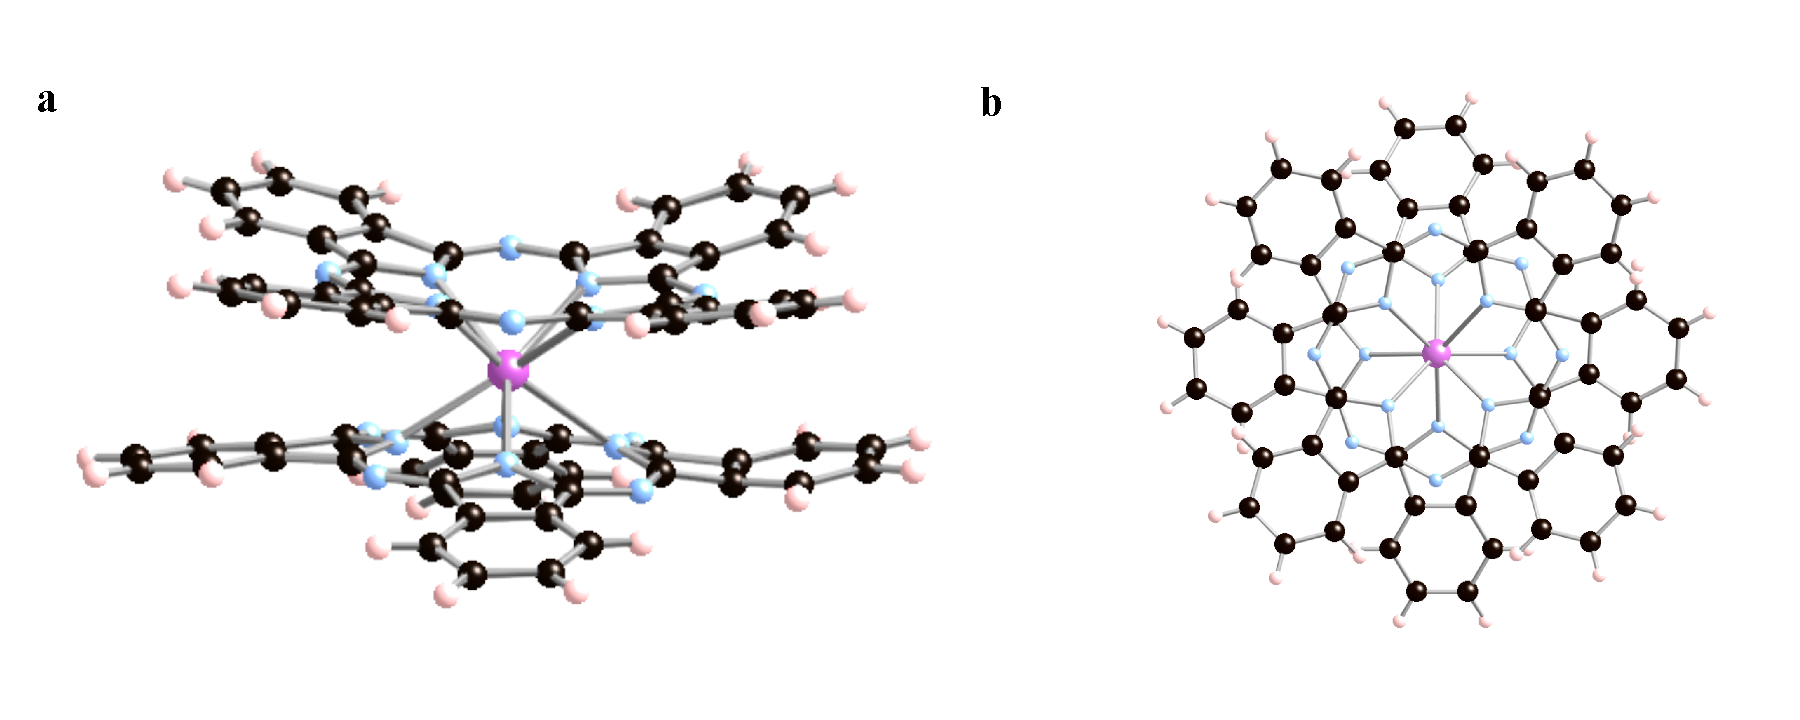
\includegraphics[scale=0.45]{Resultats/TbPc2Imag/TbPc2Imag.pdf} 
\caption{Vue d'artiste de la molécule de terbium double decker de côté~(\textbf{a}) et de dessus~(\textbf{b}). L'atome de terbium, ici en violet, est pris en sandwich entre deux phtalocyanines, ces derniers étant orientés à $45\degres$ environs, l'un par rapport à l'autre.}
\label{TbPc2Imag}
\end{figure}





\subsection{Origine du moment magnétique}
Le moment magnétique du terbium double-decker est d\^u à un centre magnétique unique : l'ion Tb$^{3+}$. L'atome de Terbium appartient à la classe des lanthanides. Son magnétisme est porté par la couche $4f$ et résulte d'un fort couplage entre le moment de spin et le moment orbital. Le moment magnétique total de l'état fondamental $J=6$ est issue, à contribution égale, du moment magnétique orbital $L=3$, et des moments magnétiques de spin des 6 électrons non appariés $S=3$. Le premier état excité $J=5$ est distant de $2900\,K$, et peut donc \^etre ignoré lorsque l'on s'intéresse aux propriétés magnétiques de la molécule.
 

\begin{figure}
\centering 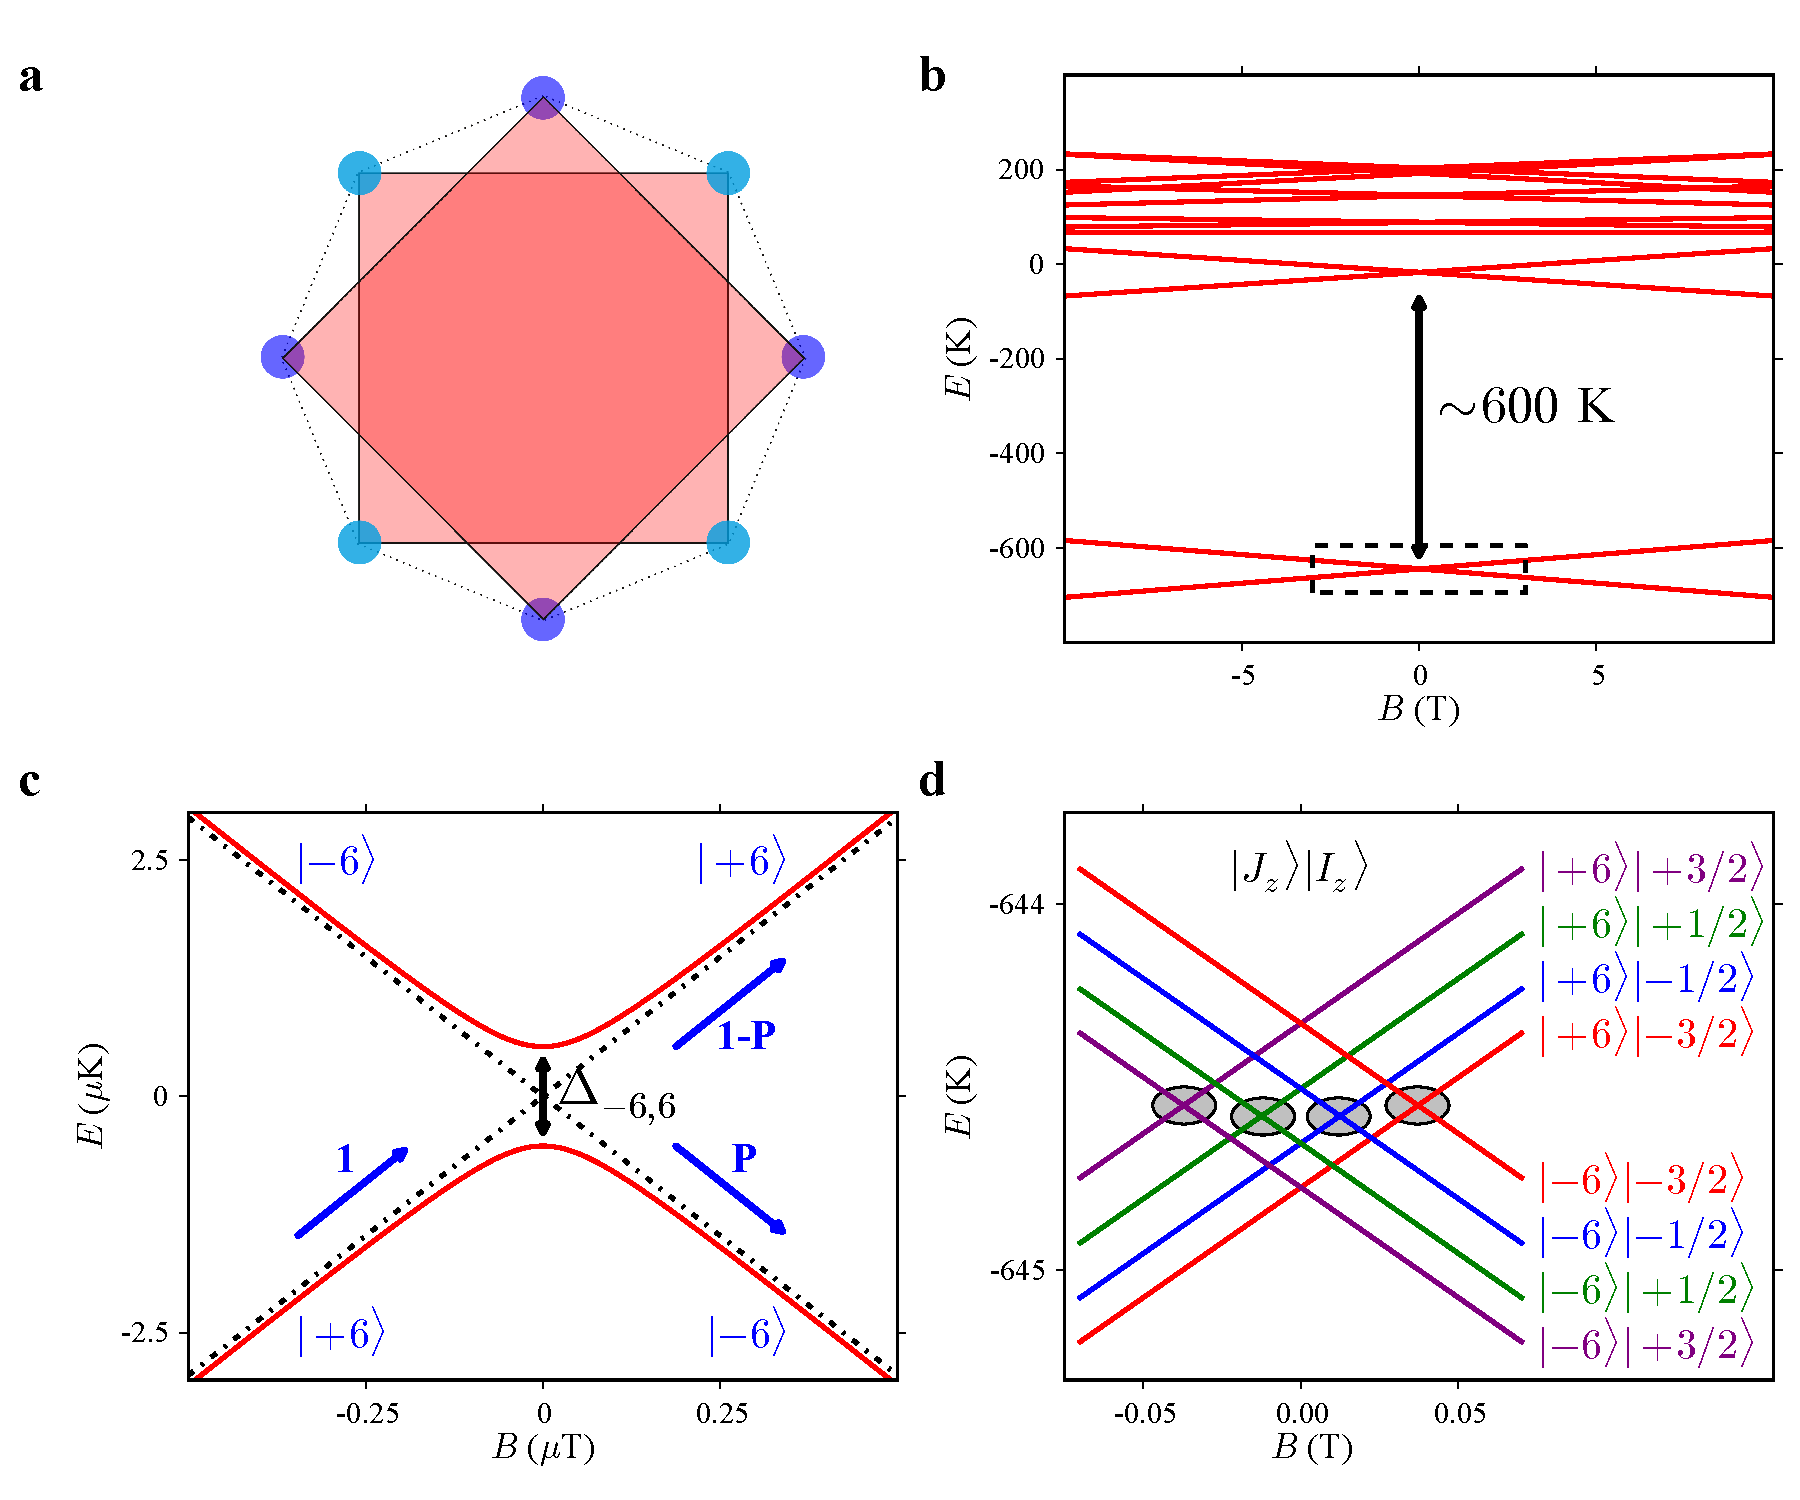
\includegraphics[scale=0.45]{Resultats/TbPc2Mag/TbPc2Mag.pdf} 
\caption{\textbf{a} : schémas représentant la coordination antiprisme. Les atomes d'azote sont représentés en bleu clair et bleu foncé, chaque couleur correspondant à un plan de ligand. \textbf{b} : diagramme Zeeman de la molécule TbPc$_2$ représentant l'énergie des différents états du système en fonction du champ magnétique. Les états fondamentaux $J_z \pm 6$ sont séparés des premiers états excités par une énergie de $600$\,K. \textbf{c} : agrandissement du diagramme Zeeman des deux états fondamentaux à faible champ magnétique. Il met en évidence un anti-croisement de valeur minimale $\Delta_{-6,6}$ de l'ordre du $\mu$K qui traduit un mélange entre les états $|+6\rangle$ et $|-6\rangle$. Si l'on balaie le champ magnétique des valeurs négatives vers les valeur positives, il existe une probabilité $P$ de passer de l'état $|+6\rangle$ à l'état $|-6\rangle$. Cette probabilité est régie par la formule de Landau-Zenner. \textbf{d} : Diagramme Zeeman lorsque l'on tient compte du couplage hyperfin entre le spin $I=3/2$ du noyau et le moment magnétique électronique. Les deux doublets sont séparés en deux jeux de quatre sous-états. On ne relève que quatre anti-croisements marqués d'un cercle, où une transition de l'état  $|+6\rangle$ à l'état $|-6\rangle$ est possible.~(inspiré de \cite{Ishikawa2005} et \cite{Sorace2011}).}
\label{TbPc2Zeeman}
\end{figure}


\subsection{Hamiltonien}

Deux contributions majeures doivent être prises en compte dans la description de la molécule TbPc$_{2}$ : la présence des ligands; le couplage hyperfin entre le moment magnétique électronique du terbium et son spin nucléaire.

\subsubsection{Le moment magnétique électronique}
Le moment magnétique de l'ion terbium est soumis à un champ de ligand définie principalement par la longueur des liaisons covalentes et la symétrie du système. 
L'ion terbium est lié de façon covalente à huit atomes d'azote, quatre pour chaque phatlocyanide. La géométrie des deux ligands, orientés à $45\degres$ l'un par rapport à l'autre, selon un axe perpendiculaire au plan des ligands, correspond à une coordination dite anti-prisme~(cf Fig.\ref{TbPc2Zeeman}.\textbf{a}). 

On peut rendre compte de cette coordination à l'aide des opérateurs de Stevens $O_2^0$, $O_4^0$ et $O_6^0$~\cite{Stevens1952,Sorace2011}. On obtient alors l'expression suivante :
\begin{eqnarray}
H = \alpha A_2^0 \langle r^2 \rangle O_2^0 + \beta A_4^0 \langle r^4 \rangle O_4^0 + \gamma A_6^0 \langle r^6 \rangle O_6^0
\end{eqnarray}
où $A_i^0$ sont les coéfficients relatifs à la molécule de TbPc$_2$~\cite{Ishikawa2005} et $\alpha$, $\beta$ et $\gamma$ les coéfficients introduits par Stevens~\cite{Stevens1952}. Les opérateurs $O^0_i$ sont basés sur des sommes d'opérateurs $S_z^{2n}$. La symétrie du système n'introduit pas de couplage entre les différents états magnétiques. 

Le diagramme Zeeman correspondant est donné dans la Fig.\ref{TbPc2Zeeman}.\textbf{b}. Les états fondamentaux $J_z = \pm 6$ sont isolés des états excités par une énergie de plus de $600\,K$. Cela garantie, à basse température, deux états possibles pour le système : $J_z = \pm 6$. Dans la suite de notre description, on pourra négliger les états excités.

 
Cependant, du fait des interactions $\pi - \pi$ entre ligands, l'angle entre les deux plans n'est pas exactement égal à $45\degres$~\cite{Koike1996}. Cela entraîne une brisure de symétrie, et nécessite l'introduction d'un nouveau terme dit terme transverse~\cite{Sorace2011} :
\begin{eqnarray}
H_{trans} = \beta A_4^4 \langle r^4 \rangle O_4^4
\end{eqnarray}
où la m\^eme notation a été utilisée. Ce dernier terme ne modifie pas l'allure générale du diagramme Zeeman. En revanche, il introduit un couplage entre les états  $J_z = \pm 6$ qui se traduit par la présence d'anti-croisement que nous allons détailler maintenant.

\subsubsection{Les anti-croisements}
La Fig.\ref{TbPc2Zeeman}.\textbf{c} présente un grossissement du diagramme Zeeman au niveau de l'anti-croisement repéré par le carré de la Fig.\ref{TbPc2Imag}.\textbf{b}. La ligne en pointillé correspond au diagramme Zeeman en l'absence de terme transverse. Si l'on se place loin de l'anti-croisement, les états $|+6\rangle$ et $|-6\rangle$ sont les états propres du système. Mais plus on se rapproche de l'anti-croisement, plus les états se mélangent.

Lorsque l'on balaie le champ magnétique autour d'un anti-croisement, il existe une probabilité de passer de l'état $|+6\rangle$ à l'état $|-6\rangle$ et vice-versas. Cette probabilité est régie par la formule de Landau-Zener~\cite{Zener1932} qui dépend à la fois de la séparation minimale entre les deux niveaux~$\Delta_{-6,6}$, ainsi que de la vitesse de balayage du champ magnétique~$\frac{dB_z}{dt}$. Cette probabilité peut s'exprimer de la façon suivante :
\begin{eqnarray}
P = 1 - \exp \left( -\frac{\pi \Delta^2_{m,m'}}{2 \hbar g \mu_B |m-m'|\frac{dB_z}{dt}} \right)
\end{eqnarray}
ou $P$ est la probabilité de passer de l'état $m$ à l'état $m'$, $m$ et $m'$ valant dans notre cas, respectivement $+6$ et $-6$. Si la vitesse est très faible, la probabilité de passer d'un état à l'autre tend vers un. On retrouve ici le théorème adiabatique. A l'autre bout de l'échelle, si le champ magnétique est balayé très rapidement, cette probabilité tend vers zéro. Tout se passe comme si le système n'avait pas eu le temps de ``sentir" l'anti-croisement.




\subsubsection{Le spin nucléaire}
De part leur forme, les orbitales $4f$ impliquées dans le magnétisme du terbium, favorisent le couplage hyperfin. Il est donc possible de mesurer l'influence de ce dernier sur les propriétés magnétiques de la molécule TbPc$_{2}$. Le spin nucléaire du terbium étant $I = 3/2$, on obtient en lieu et place des deux niveaux fondamentaux $J_z \pm 6$, deux jeux de quatre niveaux comme le montre la Fig.\ref{TbPc2Zeeman}.\textbf{d}. Cette interaction peut être prise en compte en introduisant le terme suivant dans l'hamiltonien~\cite{Bleaney1961} :
\begin{eqnarray}
H_{hf} = A_{hf}\mathbf{J}\mathbf{I}
\end{eqnarray}
où $\mathbf{J}$ et $\mathbf{I}$ sont respectivement le moment magnétique électronique et le spin nucléaire, $A_{hf}$ étant la constante d'interaction hyperfine. Il est important de noter que le terbium ne possède qu'un seul isotope, et donc un seul spin nucléaire possible.

Du fait de sa forme allongée, le spin nucléaire possède également un moment quadripôlaire dont on peut tenir compte par le terme suivant~\cite{Bleaney1961} :
\begin{eqnarray}
H_I = P\left(I_z^2 - \frac{1}{3}I(I+1)\right)
\end{eqnarray}
où $P$ est le moment quadripolaire du spin nucléaire. La présence de ce terme a pour conséquence de rendre l'espacement entre les différents niveaux non-uniforme. Ceci peut notamment avoir des applications dans le cadre de l'information quantique. Nous détaillerons ce dernier point plus tard, lorsque nous évoquerons les possibilités de manipulation du spin nucléaire.

Un digramme Zeeman incluant l'ensemble de ces contributions est présenté dans le diagramme Fig.\ref{TbPc2Zeeman}.\textbf{d}, pour les faibles champs magnétiques.



\subsection{Mesure de l'aimantation d'une assemblé}
Afin d'explorer les propriétés magnétiques des aimants moléculaires, plusieurs techniques sont envisageables. De manière générale, il faut tout d'abord obtenir un cristal moléculaire constitué par l'aimant moléculaire que l'on souhaite étudier. L'aimantation du cristal est ensuite mesurée en fonction du champ magnétique appliqué. Pour cela, on peut utiliser la techniques de micro-SQUID, qui a l'avantage d'autoriser les mesures sub-kelvins. Il s'agit d'un détecteur de variation de flux basé sur deux jonctions Josephson.

Lorsque l'on mesure un cristal moléculaire, la variation d'aimantation moyenne, induite par le retournement du moment magnétique des molécules qui le composent, entraîne une modification du flux traversant le microSQUID, qui peut être mesurée. A partir de cette mesure, et en considérant chaque aimant moléculaire comme isolé, on peut remonter aux propriétés magnétiques de ces derniers.

\begin{figure}
\centering 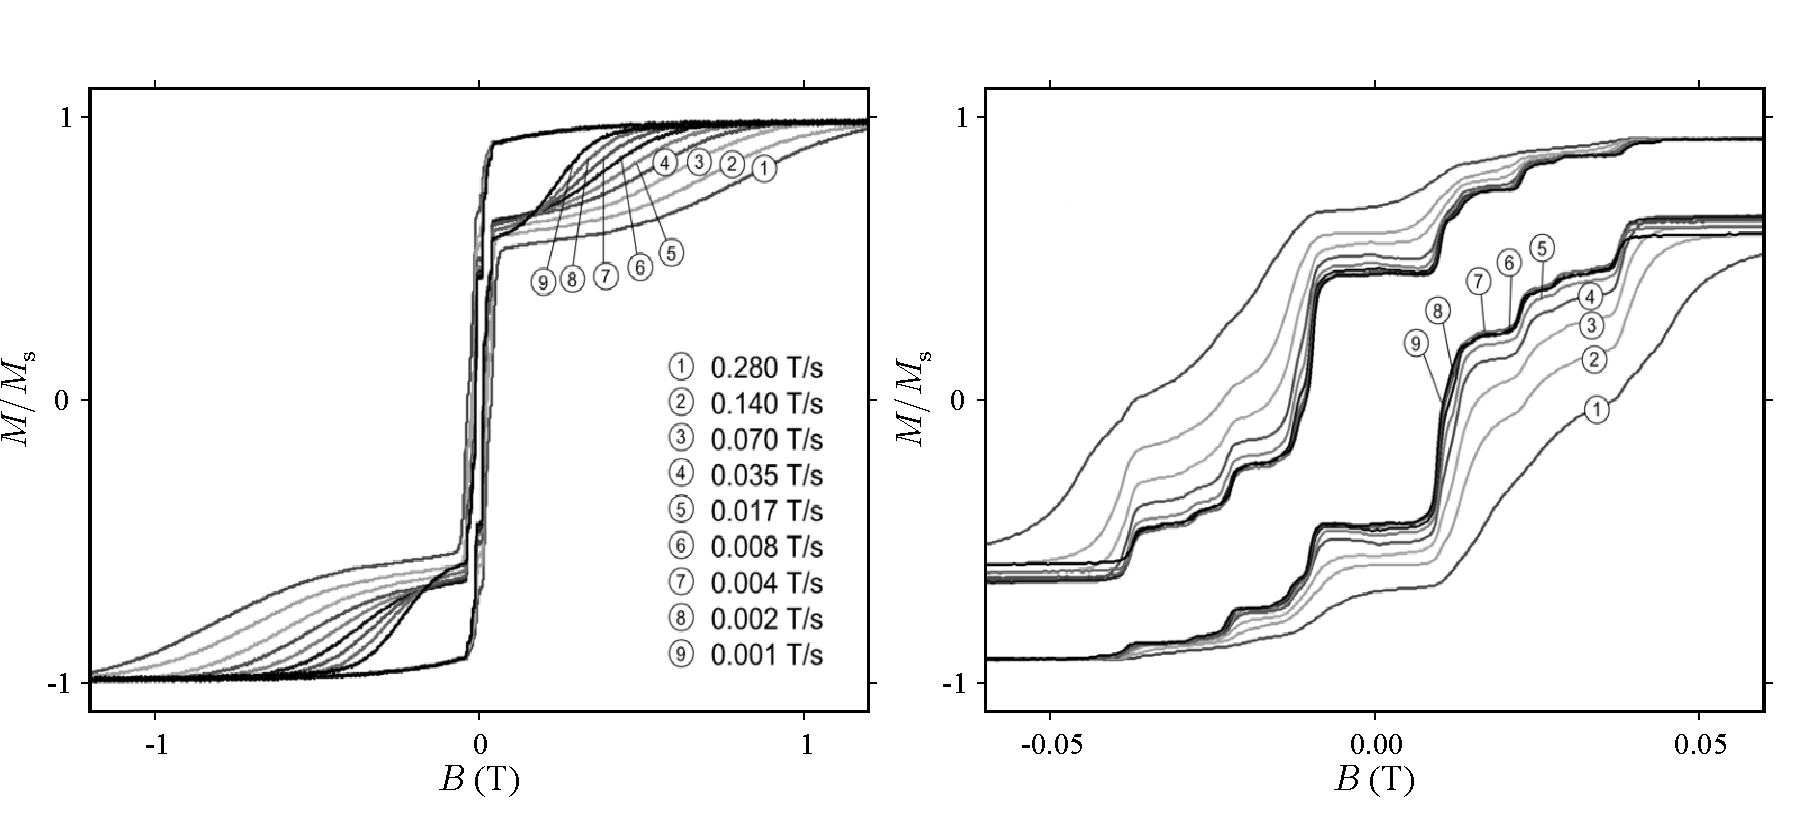
\includegraphics[scale=0.45]{Resultats/MesureAimant/MesureAimant.pdf} 
\caption{\textbf{a} : Mesure de l'aimantation d'un cristal de TbPc$_2$ à 10\,\% pour différente vitesse de balayage. \textbf{b} : grossissement de la partie centrale mettant en évidence l'influence de la vitesse de balayage sur la hauteur des marches associées au retournement par QTM.(extrait de \cite{Ishikawa2005}).}
\label{TbPc2Aimantation}
\end{figure}


Une mesure de l'aimantation d'un cristal de TbPc$_2$ pour différentes vitesses de balayage est présentée dans la Fig.\ref{TbPc2Aimantation}.\textbf{a}. Une analyse détaillée peut \^etre trouvée dans \cite{Ishikawa2005}. On peut diviser la courbe en deux zones. 

A faible champ~(cf Fig.\ref{TbPc2Aimantation}.\textbf{b}), les molécules constituant le cristal se retournent par QTM. Les marches rendent compte du retournement de l'aimantation au niveau des anti-croisements présentés dans la Fig.\ref{TbPc2Zeeman}.\textbf{d}. Ce dernier est gouverné par la formule de Landau-Zener. Il dépend donc de la vitesse, ce qui conduit à une variation de la hauteur des marches en fonction de la vitesse de balayage, comme le montre la Fig.\ref{TbPc2Aimantation}.\textbf{b}. 

A plus fort champ, l'aimantation ne peut se retourner qu'en émettant un phonon. La position en champ magnétique de ces retournements direct dépend donc de la distribution en énergie des phonons du système, d'où la zone de transition continue. L'influence de la vitesse de balayage est dans ce cas liée à un effet que l'on nomme Phonon-Bottleneck~\cite{VanVleck1941}. Elle rend compte du fait que les moments magnétique d'un trop grand nombre de molécules ``souhaitent" se retourner pour que toutes puissent émettre un phonon.

\subsection{TbPc$_2$ et la spintronique}
Pour qu'un aimant moléculaire puisse être utilisé dans le cadre de la spintronique moléculaire, il doit remplir plusieurs critères : il doit conserver ses propriétés magnétiques lorsqu'il est déposé sur une surface métallique; dans le cas de l'électromigration, il doit pourvoir résister à des température de plusieurs centaine de degrés Celsius; enfin, il doit être relativement robuste vis à vis de la déformation.

\begin{figure}
\centering 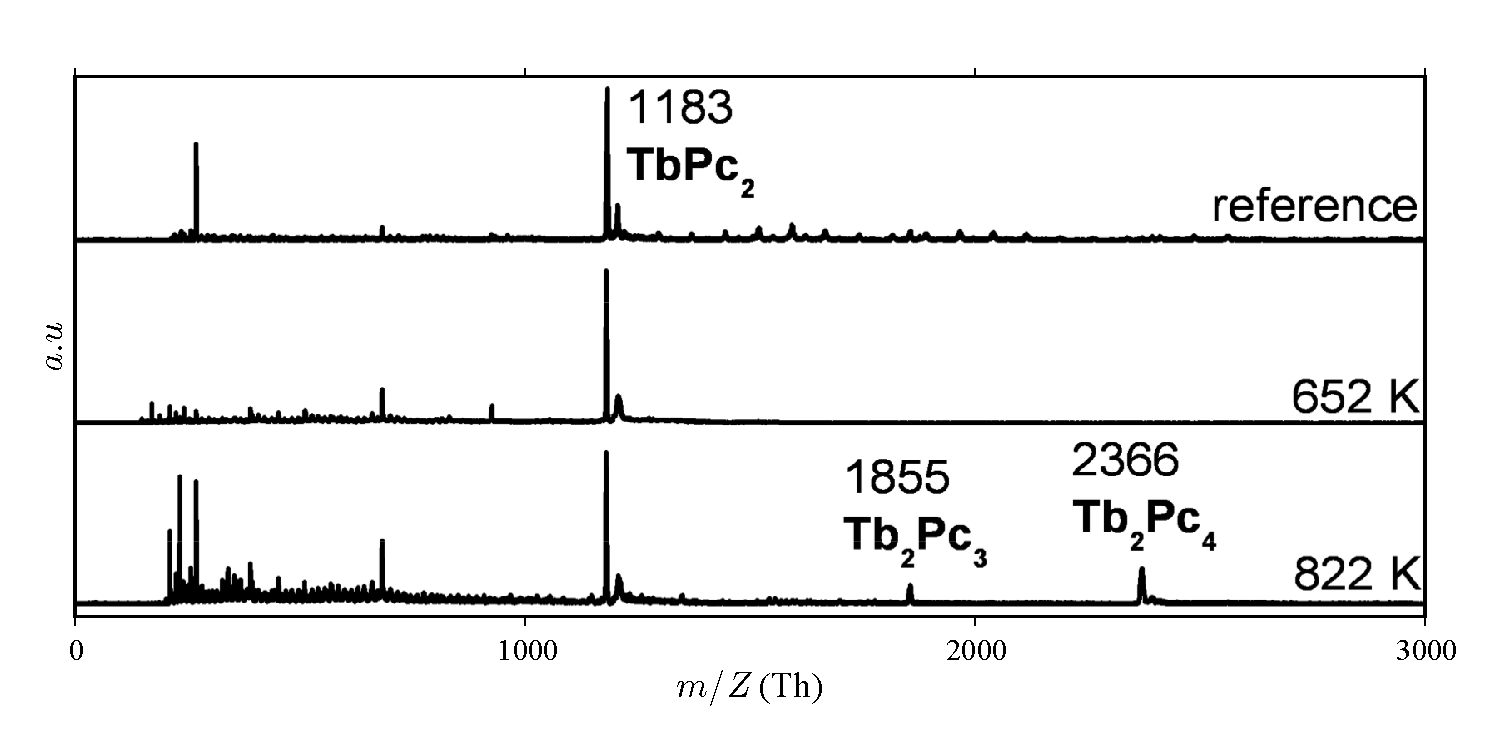
\includegraphics[scale=0.45]{Resultats/TbPcResTemp/TbPcResTemp.pdf} 
\caption{Spectromètre obtenue par évaporation à différente température d'une poudre de TbPc$_2$. Un échantillon de cette même poudre dissoute dans du dichlormethane et de l'ethanol à servi de référence. (extrait de ??).}
\label{SpectMass}
\end{figure}

L'analyse des propriétés magnétique du TbPc$_{2}$ sur des surfaces de cuivre a été étudié par XMCD~(X-ray Magnetic Circular Dichroism). Cette étude a confirmé la robustesse des propriétés magnétiques vis à vis de l'adsorption sur une surface conductrice. De plus, la technique de déposition impliquait de chauffer la poudre d'aimant moléculaire à des température de plusieurs centaines de degrés. Une analyse au spectromètre de masse a montré que la structure du TbPc$_{2}$ pouvait demeurer intacte jusqu'à une température de $820\,K$~(cf Fig.\ref{SpectMass}). Enfin, si elle reste sensible aux déformations en compression, elle se montre en revanche peut dépendante de la déformation en torsion~\cite{Sorace2011}, cette dernière ne venant modifier que légèrement le terme $A_4^4 \langle r^4 \rangle$ dans la description du système~(et donc la probabilité de retournement par QTM).

Cet aimant moléculaire a, en outre, l'avantage de mettre en jeux magnétisme électronique et magnétisme nucléaire, ce qui rend la physique plus riche, et donc les applications éventuelles plus nombreuses. D'autant que le terbium ne possède qu'un seul isotope, ce qui garantit les mêmes propriétés magnétiques, quelque soit l'aimant moléculaire.

\section{Magnétisme et transport}
Afin de comprendre comment le magnétisme moléculaire peut se coupler au transport électronique, il est nécessaire d'identifier les mécanisme régissant ce dernier, dans le cas de structure nanométriques. La première partie de ce section sera consacré à cette étude.
Puis, nous décrirons comment ces mécanismes peuvent \^etre sensibles au moment magnétique d'une molécule unique, à travers deux configurations différentes. Enfin, nous aborderons les différents interactions permettant de coupler le magnétisme moléculaire et le transport mésoscopique.

\subsection{Transport à travers une boite quantique}
Une boite quantique peut se définir comme un système de petite taille, dans lequel les niveaux énergies sont discrets. Lorsque l'on couple un boite quantique à deux électrodes conductrices, on obtient la configuration de la Fig.\ref{DotSchem}.\textbf{a}, où des niveaux d'énergie discrets sont séparés du continuum d'état des électrodes par une barrière tunnel définie par les paramètre $\gamma_i$, et le couplage capacitif $C_i$~($i=s$ pour la source et $i=d$ pour le drain).

En appliquant une tension source-drain, on ouvre une fenêtre de potentiel chimique. Si le potentiel chimique du point quantique se situe en dehors de cette fen\^etre, l'état de charge de la boite est défini, et aucun courant ne traverse le système~(cf Fig.\ref{DotSchem}.\textbf{a}). En revanche, si ce dernier se trouve cette fen\^etre, alors un courant est mesuré, et les électrons peuvent circuler en passant, un à un, à travers l'\^ilot central~(cf Fig.\ref{DotSchem}.\textbf{b}). 

\begin{figure}
\centering 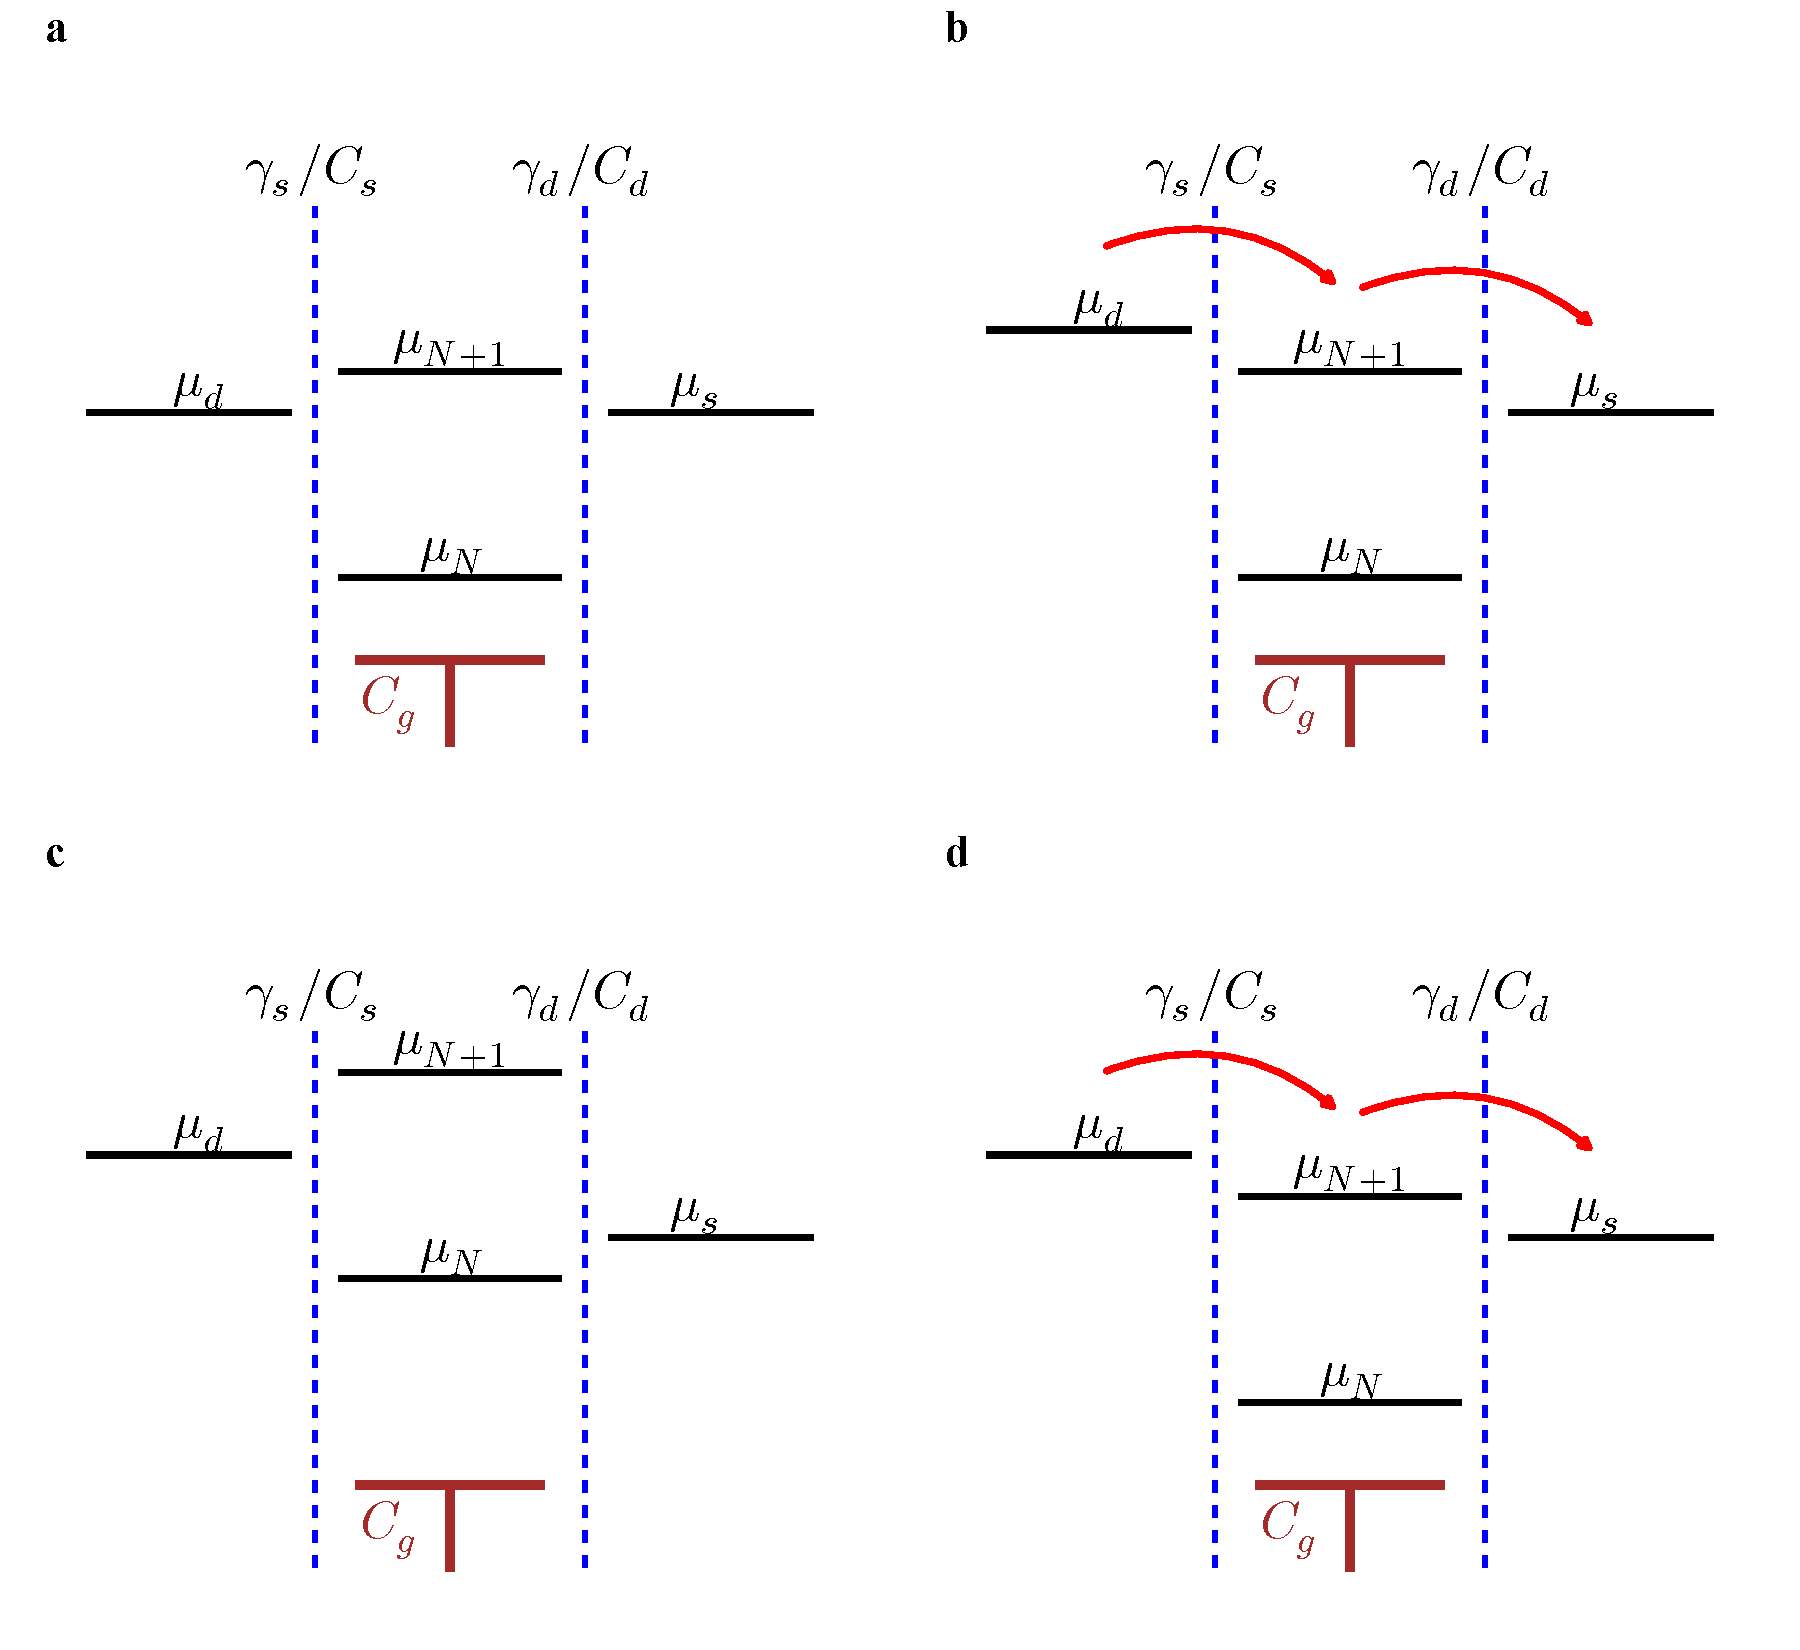
\includegraphics[scale=0.45]{Resultats/DotSchem/DotSchem.pdf} 
\caption{Représentation schématique d'une boite quantique. \textbf{a} : Lorsque les potentiels chimique de la source et du drain~($\mu_s$ et $\mu_d$) ne sont pas alignés avec ceux du point quantique, aucun courant ne circule, et l'état de charge du point quantique est bien défini~(ici N). \textbf{b} : en appliquant une tension source drain, on ouvre une fenêtre de potentiel chimique. Si le potentiel chimique du point quantique se trouve dans cette fenêtre, un courant peut circuler. De plus, en appliquant une tension sur l'électrode de grille, on peut amener un potentiel chimique, initialement en dehors de la fenêtre~(\textbf{c}), à l'intérieur de celle-ci~(\textbf{d}), induisant un courant.}
\label{DotSchem}
\end{figure}


Afin de pouvoir moduler le potentiel chimique de la boite quantique, on peut ajouter une électrode de grille qui ne vas être couplé, de manière capacitive, à cette dernière. En appliquant une tension sur cette électrode, l'échelle des potentiels chimiques peut être décalée, et donc, le courant modulé. On peut ainsi passer d'une situation où le courant est nul~(cf Fig.\ref{DotSchem}.\textbf{c}), à une situation ou les électrons peuvent circuler~(cf Fig.\ref{DotSchem}.\textbf{d}).

On peut maintenant imaginer deux configurations. Dans la première, la boite quantique est définie par la centre magnétique, et ce dernier va osciller entre deux états de charge, et donc, deux configuration magnétique~(cf Fig.\ref{DirVsInd}.\textbf{a}). 
Dans la deuxième configuration, la boite quantique n'est pas confondue avec le centre magnétique, mais seulement couplée magnétiquement à ce dernier~(cf Fig.\ref{DirVsInd}.\textbf{b}). Dans la suite, la première configuration sera qualifiée de configuration directe, et la seconde, de configuration indirecte.


\subsection{La configuration directe}
Le couplage direct implique que les électrons responsables du courant, jouent également un rôle dans le magnétisme de la molécule. Cette dernière va osciller entre deux états de charge N/N+1 , chacun d'eux ayant sa propre configuration magnétique $S_N$ et $S_{N+1}$~(cf Fig.\ref{DirVsInd}.\textbf{a}). L'analyse se fait en sondant la différence en énergie des différentes transitions N/N+1~(i.e. la position des potentiels chimiques associés à chaque transition), le plus souvent, par une technique de spectroscopie en tunnelling séquentiel~(cf annexe sur le transport mésoscopique). Celle-ci a l'avantage de donner accès à différents états de charge~(nombre d'oxydation ou de réduction). En revanche, le caractère très invasif de la méthode ne laisse pas espérer de long temps de vie pour les différents états du système. Cette dernière a été mise en œuvre expérimentalement dans \cite{Heersche2006,Jo2006,Zyazin2010} avec des résultats mitigés, du fait notamment de la dégradation de la molécule lors de la fabrication du dispositif~\cite{Jo2006}. Des études théoriques ont également été menées~\cite{Timm2006,Timm2007}, permettant une analyse plus fine des résultats expérimentaux.

\subsection{La configuration indirecte}

Dans le cas du couplage indirect, les électrons responsables du courant ne participent qu'indirectement au magnétisme de la molécule~(cf Fig.\ref{DirVsInd}.\textbf{b}). Comme nous le montrerons dans la suite, la mesure se fait par l'analyse statistique des modifications de conductance du système en fonction du champ magnétique. La polarisation en tension source-drain et grille est, en général, fixée~(par opposition à la spectroscopie en tunneling séquentiel). Dans cette configuration, le nombre d'électrons impliqués dans le magnétisme moléculaire ne peut pas être modifié. En revanche, la technique de mesure en configuration indirect, se révèle beaucoup moins invasive. Cela garantie, d'une part, la préservation des propriétés magnétiques, et d'autre part, l'observation de longs temps de vie. 

Cette configuration a été utilisée dans deux dispositifs légèrement différents. Dans le premier, une deuxième molécule~(un nanotube) a été utilisée comme point quantique sonde, l'aimant moléculaire étant déposé sur sa surface \cite{Urdampilleta2011}. Dans le deuxième dispositif, une seule molécule a été utilisée. Le cœur magnétique de cette dernière étant fortement découplé des ligands périphériques, ils ont pu être utilisé comme point quantique sonde~\cite{Vincent2012}. Cette dernière configuration correspond au dispositif que nous nous proposons d'étudier dans la suite. Quelques outils théoriques sont venus faciliter l'interprétation des résultats [papier sur nanotube], mais également proposer de nouvelles expériences~\cite{Jaafar2010} +[article du les ligand qu'il faut que je retrouve..].


\begin{figure}
\parbox{6.5cm}{
\centering 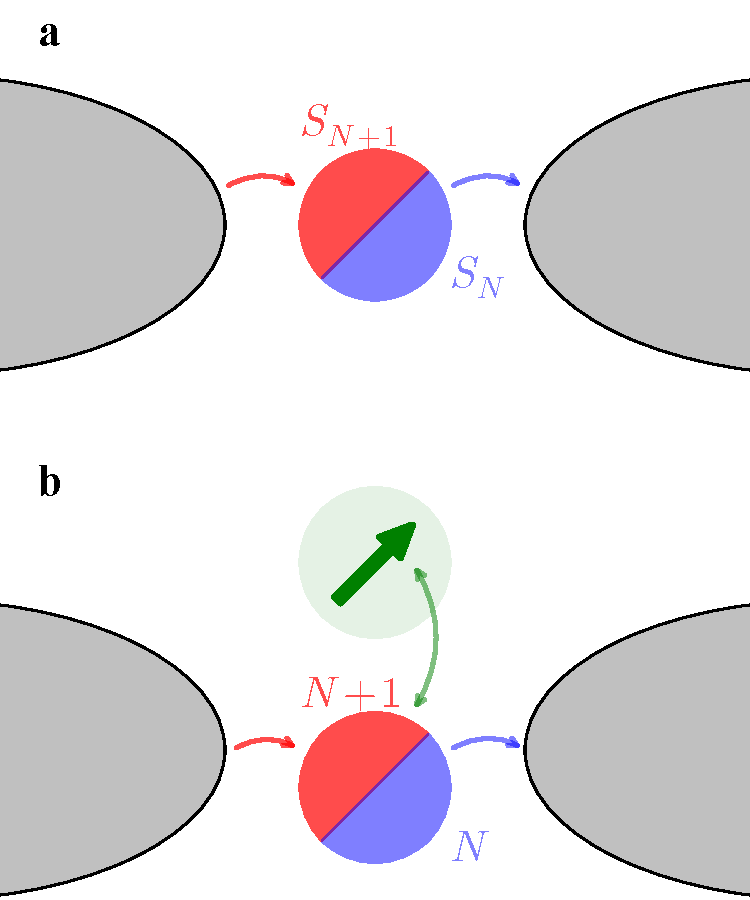
\includegraphics[scale=0.45]{Resultats/DirVsInd/DirVsInd.pdf} 
}
\parbox{7.5cm}{
\caption{\textbf{a} : configuration directe. Le centre magnétique est directement impliqué dans le transport électronique. Il oscille entre les états de charges $N$ et $N+1$. Cette oscillation entraîne une alternance entre les états magnétiques $S_{N}$ et $S_{N+1}$. \textbf{b} : configuration indirecte. Le centre magnétique n'est pas directement couplé au transport électronique mais par l'intermédiaire d'une boite quantique. Cette dernière oscille entre deux états de charge $N$ et $N+1$, ces derniers étant influencé par l'état magnétique du centre magnétique, du fait d'une interaction~(exchange, dipolaire etc.).}
\label{DirVsInd}
}
\end{figure}


\subsection{Le couplage magnétisme-transport}
Dans la configuration directe présentée précédemment, le couplage entre le courant et le magnétisme est aisé à comprendre, les électrons participant au premier étant également directement impliqués dans le second. En revanche, dans la configuration indirecte, le couplage entre ces deux domaines peut avoir plusieurs origines. Il a pour conséquence de rendre l'énergie du point quantique, et donc son potentiel chimique, dépendante de l'état du centre magnétique. Cette dépendance est fonction de la nature de l'interaction, comme nous allons le montrer maintenant.

\subsubsection{Le couplage dipolaire}

\begin{figure}
\parbox{6.5cm}{
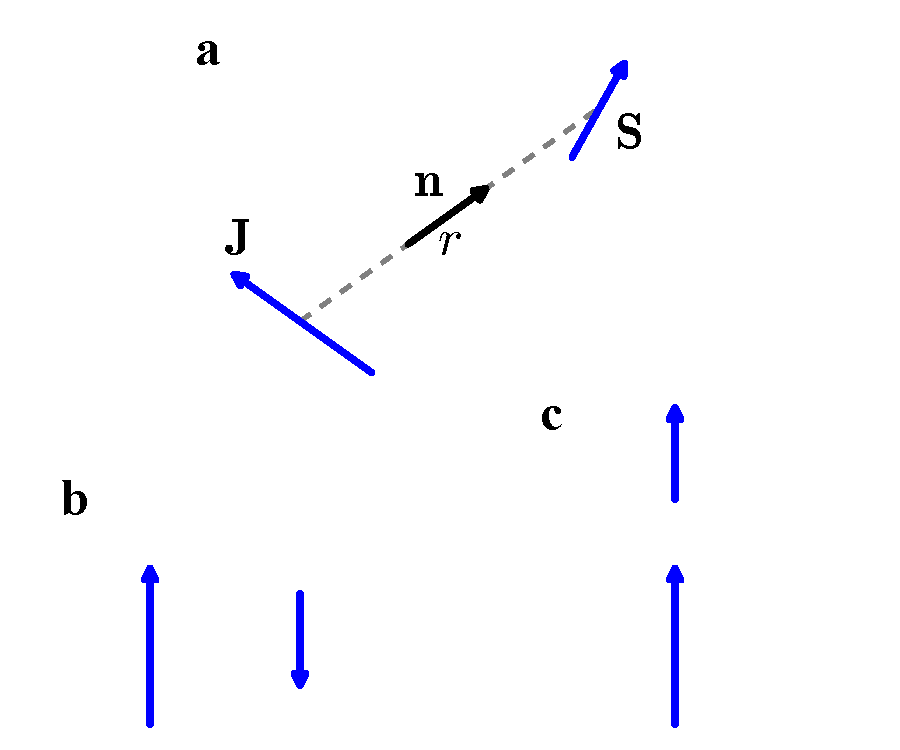
\includegraphics[scale=0.45]{Resultats/CDipolaire/CDipolaire.pdf} 
}
\parbox{7cm}{\caption{\textbf{a} - Schéma représentatif du couplage dipolaire entre deux spins \textbf{J} et \textbf{S} séparés par une distance $r$. \textbf{b}(\textbf{c}) - configuration anti-ferromagnétique~(ferromagnétique) induite par le couplage dipolaire. Dans le cas du TbPc$_2$, l'axe facile étant perpendiculaire au plan des ligands, la configuration \textbf{c} est la configuration la plus vraisemblable.}
\label{dipolaire}
}
\end{figure}


Le couplage dipolaire est une interaction à distance entre deux moments magnétiques. Chacun de ces moments génère un champ dipolaire qui va venir agir sur le second, et vice versa. La modification en énergie induite est fonction de la distance séparant les deux dipôles, ainsi que de leur orientation relative. Ceci s'exprime par:
\begin{eqnarray}
E = -\frac{\mu_0^2 \mu_B^2}{4\pi r^3}(3\mathbf{SnJn} - \mathbf{SJ}) \nonumber
\end{eqnarray}
où $\mathbf{S}$ et $\mathbf{J}$ sont les spins associés aux deux moments magnétiques, $r$ la distance qui les sépare et $\mathbf{n}$ la normale reliant les deux moments (cf Fig.\ref{dipolaire}.a). En terme d'opérateur, cette expression peut se réécrire :
\begin{eqnarray}
E = -\frac{\mu_0^2 \mu_B^2}{4\pi r^3}(1 - 3 \cos^2 \theta) \lbrace S_zJ_z - \frac{1}{4}(J_+S_- + J_-S_+)\rbrace \nonumber
\end{eqnarray}
où $\theta$ est l'angle entre les deux spins.

Plusieurs remarques s'imposent. Premièrement, l'intensité de l'interaction est proportionnelle à l'inverse de la distance au cube. Elle devient très rapidement négligeable : pour un spin $J=6$, elle ne vaut plus que $10$\,mT à $1$\,nm. Deuxièmement, en fonction de l'angle $\theta$, on peut imaginer deux configurations opposées : dans la situation de la Fig.\ref{dipolaire}.b, le couplage abouti à une organisation anti-ferromagnétique; dans celle présentée dans la Fig.\ref{dipolaire}.c, le couplage est au contraire ferromagnétique.

La seule transition possible à basse température est $J_z=\pm6 \rightarrow J_z \mp 6$. En conséquence, la variation du potentiel chimique du point quantique sonde $\mu_{QD}$ est liée au renversement du moment magnétique par :
\begin{eqnarray}
\Delta \mu_{QD} = -\frac{\mu_0^2 \mu_B^2}{2\pi r^3}S_z\Delta J_z(1 - 3 \cos^2 \theta)   \nonumber
\end{eqnarray}
Celle-ci est directement proportionnelle à $\Delta J_z$.


\subsubsection{Le couplage d'échange}
Le couplage d'échange est une interaction de contact entre deux moments magnétiques. Il résulte d'un recouvrement des fonctions d'onde et peut favoriser deux situations opposées : si l'interaction est de type ferromagnétique, les spins s'alignent entre eux ; si elle est de type anti-ferromagnétique, l'orientation entre spin est opposée. Cette interaction s'exprime comme suit :
\begin{eqnarray}
E = A\mathbf{SJ} \nonumber
\end{eqnarray}
où $A$ est la constante d'échange. Lorsque $A>0$, le couplage est anti-ferromagnétique, si $A<0$, il est ferromagnétique. La constante d'échange peut prendre des valeurs élevées en énergie : dans le cas du N@C$_{60}$ par exemple, la valeur de l'échange entre le spin de l'azote et les électrons du C$_{60}$ a été mesurée comme étant supérieure à 4\,T~\cite{Roch2011}. Si l'on tient compte des considérations évoquées dans le cas du couplage dipolaire, la modification d\^u à l'interaction d'échange qu’entraîne un retournement de l'aimantation peut s'exprimer de la façon suivante :
\begin{eqnarray}
\Delta \mu_{QD} = AS_z\Delta J_z\nonumber
\end{eqnarray}
Cette expression est semblable à celle obtenue pour le couplage dipolaire. La principale différence réside dans l'intensité de l'interaction : si celle-ci est de l'ordre du $mT$, elle est certainement dipolaire; si elle est de quelques dizaines de $mT$, l'interaction d'échange est certainement l'interaction dominante.

\subsubsection{Le couplage magnéto-Coulomb}
L'origine de ce couplage est électrostatique. Il a été mis en évidence par~\cite{Molen2006} dans les valves de spin, puis étudié dans le cas de nanotubes couplés à des particules magnétiques dans~\cite{Datta2011}. Si l'on considère un point quantique et un centre magnétique, cette interaction va coupler le potentiel chimique du premier à celui du second de telle sorte que :
\begin{eqnarray}
\Delta \mu_{QD} = C_{mc} \Delta \mu_{CM}
\end{eqnarray}
où $C_{mc}$ est la constante de couplage et $\Delta \mu_{CM}$ la variation du potentiel chimique du centre magnétique. Cette expression peut être simplifiée, au regard des remarques précédentes, de la façon suivante :
\begin{eqnarray}
\Delta \mu_{QD} = C_{mc} g \mu_B  \Delta J_z B_z
\end{eqnarray}
Contrairement aux expressions précédentes, la variation du potentiel chimique associée à un retournement de l'aimantation n'est pas constante mais dépend du champ magnétique appliqué, ce qui rend cette dernière, facile à identifier.


Après avoir cerné les mécanismes pouvant être en jeux dans notre système, nous allons maintenant nous consacrer à l'étude détaillé de ses propriétés. Pour cela, nous allons présenterons rapidement la signature transport de ce dernier, puis nous analyserons en détail le ou les mécanismes, responsables du couplage entre magnétisme et transport électronique.

\section{Description de notre échantillon}
Avant de procéder à l'étude du magnétisme moléculaire, il est important de comprendre comment ce dernier interagit avec les électrons impliqués dans le transport. Il nous faut, pour cela, identifier la configuration de notre échantillon : directe ou indirecte. Ensuite, il est nécessaire de caractériser la ou les interactions assurant le couplage entre magnétisme et transport électronique.


\subsection{Signature en transport}

Avant d'étudier en détail la réponse magnétique de notre système, il est important de savoir si l'on se trouve en configuration directe ou indirecte. La première est généralement rencontrée lorsque l'on piège une molécule au sein d'un interstice nanométrique, constitué par les électrodes de source et de drain.

Dans le cas du TbPc$_{2}$, cette hypothèse est cependant peut vraisemblable. En effet, une configuration directe signifie que l'on modifie le nombre d'électrons impliqués dans le magnétisme. Dans notre cas, cela reviendrait à changer le nombre d'électron de la couche $4f$ de l'atome de terbium, et requerrait une énergie de l'ordre de l'électron-Volt. On s'attend donc à obtenir une configuration indirecte.

\begin{figure}
\parbox{7cm}{
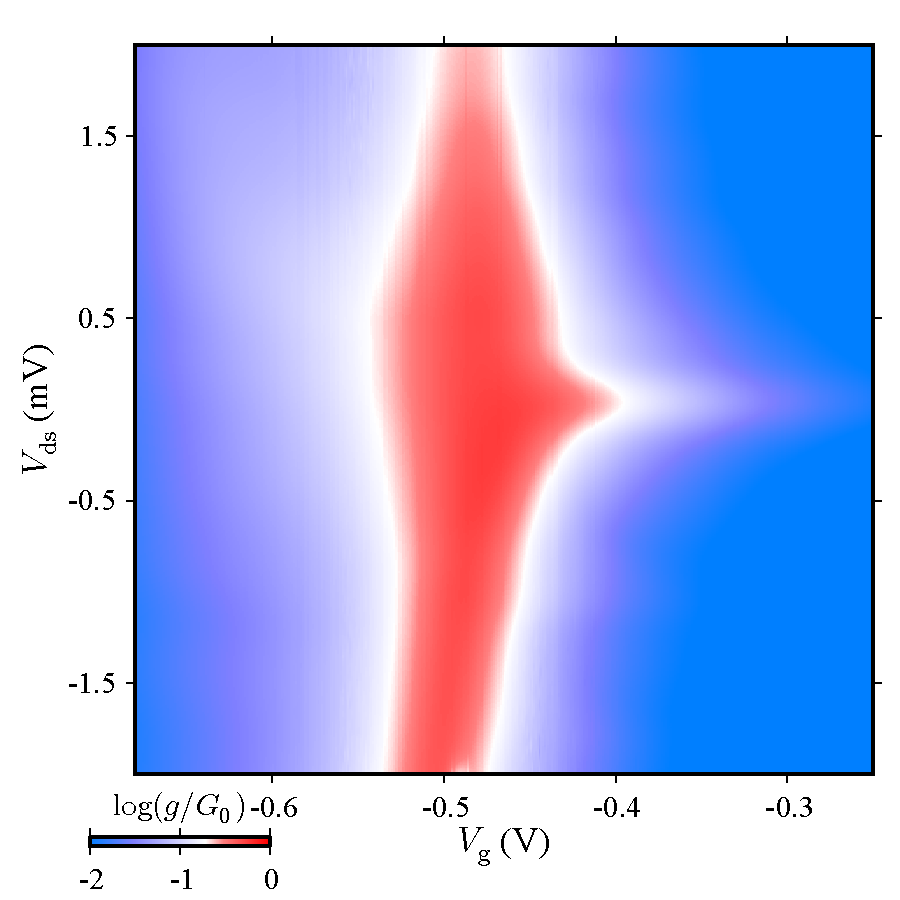
\includegraphics[scale=0.45]{Resultats/CoulombMap/CoulombMap.pdf} 
}
\parbox{6.5cm}{\caption{Digramme de Coulomb montrant la mesure en conductance différentielle de notre échantillon, en fonction de la tension de grille $V_{\rm{g}}$ et la tension source drain $V_{\rm{ds}}$.}
\label{coulomb_map}
}
\end{figure}

Afin de confirmer cette hypothèse, nous avons mesuré la conductance différentielle de notre échantillon en fonction des tensions source-drain et de grille. La Fig.\ref{coulomb_map} présente le diagramme de stabilité obtenu dans lequel un pic de conductance est observable pour $V_{\rm{g}}=-0.5\,V$. Celui-ci correspond à un changement d'état de charge de notre point quantique, ce dernier étant de $N$ à gauche et de $N+1$ à droite. Le diamant de Coulomb habituellement rencontré dans ce type de mesure n'est pas visible ici, certainement du fait d'un fort couplage au électrode,ainsi qu d'un couplage tunnel asymétrique entre la source et le drain.

Un élément important de cette mesure, est la présence d'une résonance à tension source-drain nulle, du côté droit du point de dégénérescence. Elle traduit la présence d'un moment magnétique sur notre point quantique, ce dernier venant interagir avec les électrons de la source et du drain : c'est l'effet Kondo~\cite{Kondo1964,Wilson1975,Goldhaber-Gordon1998}.
 Il a été initialement observé dans les matériaux massifs contenant des impuretés magnétiques, ces dernières venant se coupler aux électrons de conduction. Dans notre cas, l'impureté magnétique n'est rien d'autre que le moment magnétique de notre point quantique, les électrons de conduction provenant de la source et du drain. Ce couplage étant anti-ferromagnétique, l'effet Kondo à pour conséquence de venir ``écranter'' le moment magnétique.

Lorsque l'on traite ce phénomène dans le cas de boites quantiques, on peut en rendre compte par une densité d'état élevé au niveau de fermi de la source et du drain. Elle donne lieu à la résonance en conductance différentielle, à tension source-drain nulle~\cite{Goldhaber-Gordon1998}, que nous observons dans nos mesures.

Lorsque l'on applique un champ magnétique sur une résonance Kondo, il est possible de la scinder en deux, une à tension positive et l'autre à tension négative, comme le montre la Fig.\ref{analyse_interaction}.\textbf{d}. En analysant l'évolution de ces dernières, et notamment la pente à champ magnétique élevé, il est possible d'en déduire la nature du moment magnétique. Dans notre mesure, on retrouve l'écart Zeeman correspondant à un spin $1/2$, ce dernier étant simplement décalé comme nous le verrons dans la suite.

La présence de ce spin $1/2$ signifie tout d'abord que le transport n'implique pas directement notre centre magnétique dont le moment magnétique est de $6$. Il correspond à une boite quantique dont le niveau électronique est à motié rempli, laissant le spin de l'électron non apparié interagir avec les électrons de la source et du drain. Les états de charge du système sont $N=0$ à gauche du point de dégénérescence et $N=1$ à droite. De plus, comme nous allons le voir dans la suite, notre système est sensible au magnétisme de l'atome de terbium. \textbf{Nous sommes donc dans une configuration indirecte}. Dans ce cadre, on peut envisager trois interactions responsables du couplage entre notre centre magnétique et notre point quantique sonde : magnéto-Coulomb, couplage d'échange, et couplage dipolaire.

Nous allons maintenant identifier quels sont la ou les interactions réellement en jeu.

\subsection{Amplitude des sauts de conductance}
Précédemment, nous avons montré que le courant traversant le système, et donc, la conductance différentielle mesurée $g$, était directement relié au potentiel chimique du point quantique. On peut résumer cette tendance par la relation suivante:
\begin{eqnarray}
\text{d}g = \frac{\partial g}{\partial \mu} \text{d} \mu
\end{eqnarray}
Lorsque $\frac{\partial g}{\partial \mu} = cst$, la variation observée en conductance est une mesure directe de la variation du potentiel chimique. De plus, en raison de l'effet Zeeman, le potentiel chimique varie linéairement avec le champ magnétique, de sorte que $\text{d}\mu \propto \text{d}B$. Pour avoir une lecture directe de la variation du potentiel chimique, il faut donc choisir un point de fonctionnement tel que $\frac{\partial g}{\partial B} = cst$. La Fig.\ref{analyse_interaction}.\textbf{a} montre une mesure de $g$ en fonction du champ magnétique $B$, et met en évidence les zones correspondantes. Dans ces zones, un saut en conductance est directement proportionnel à la variation du potentiel chimique. 

La mesure présentée dans Fig.\ref{analyse_interaction}.\textbf{b} montre clairement que la hauteur des sauts en conductance, et donc la variation du potentiel chimique, ne dépendent pas du champ magnétique. Or, \textbf{cette observation n'est pas compatible avec une interaction de type magnéto-Coulomb}, ce qui nous permet de l'exclure des mécanismes de coulage. On a donc à faire, soit à un couplage dipolaire, soit à un couplage d'échange. Seule l'analyse de l'intensité de l'interaction peut nous renseigner. C'est à sa détermination que nous allons nous attacher maintenant.

\begin{figure}
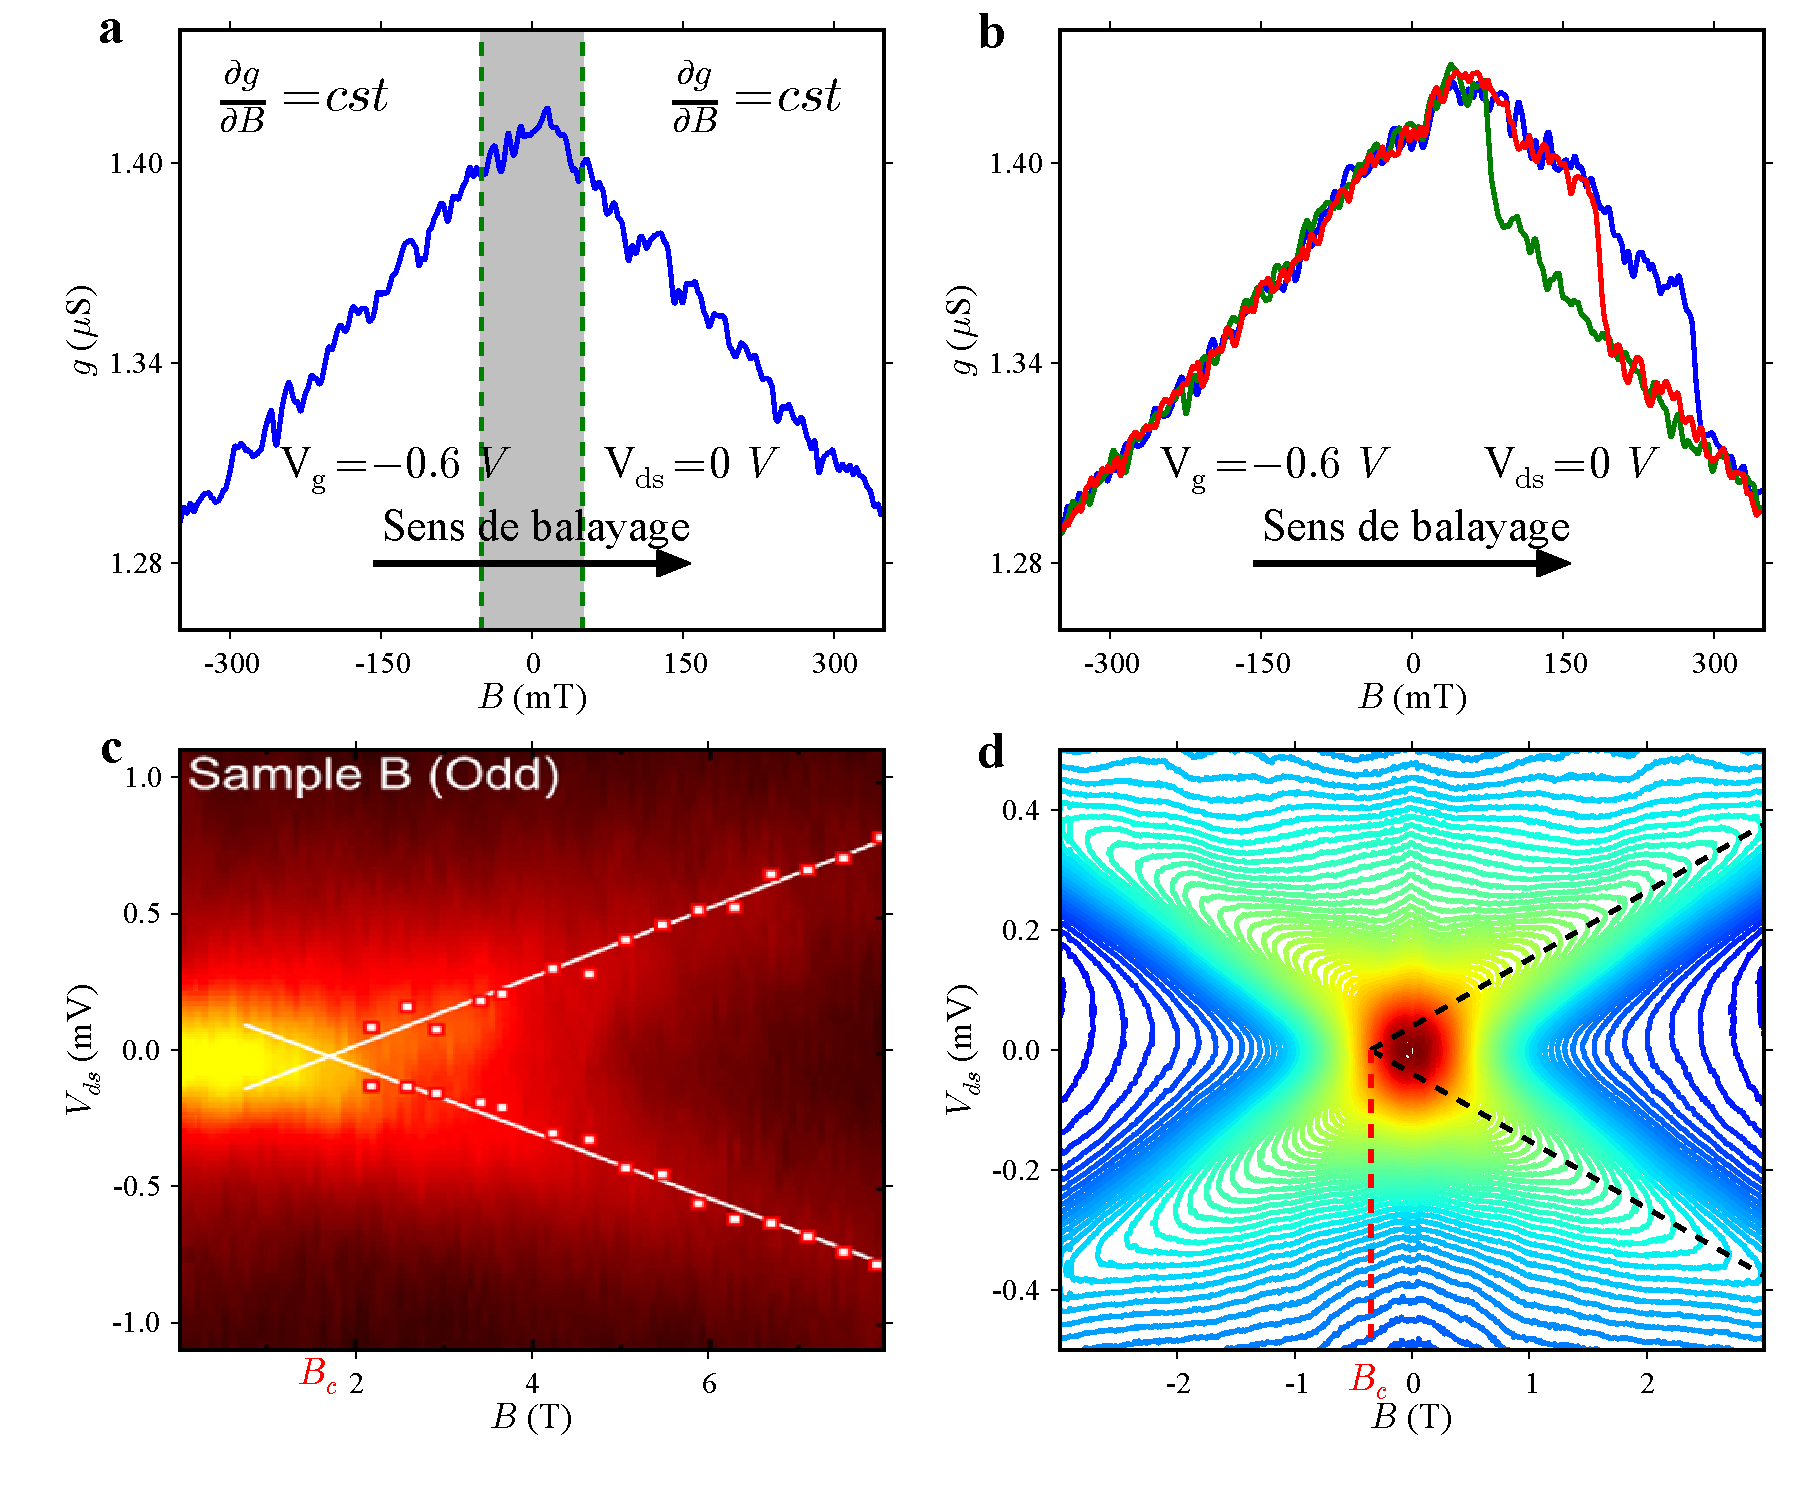
\includegraphics[scale=0.45]{Resultats/AmplJump/AmplJump.pdf} 
\caption{\textbf{a} - Mesure en conductance différentielle en fonction du champ magnétique en l'absence de saut de conductance : les zones non grisées correspondent à des valeurs de champ magnétique où la variation de potentiel chimique $\Delta \mu$ est directement proportionnelle à la variation en conductance $\Delta g$. \textbf{b} - Mesure de trois sauts de conductance pour différentes valeurs de champ magnétique : celle-ci met en évidence l'indépendance de la variation $\Delta g$ vis à vis du champ magnétique appliqué. \textbf{c}(\textbf{d}) : Mesure en conductance différentielle de l'effet Kondo 1/2 en fonction du champ magnétique et de la tension source-drain pour un système sans~(soumis à l') interaction d'échange. L'extrapolation des maxima de conductance permet d'extraire la séparation Zeeman ainsi que la valeur du champ critique $B_c$.}
\label{analyse_interaction}
\end{figure}

\subsection{Intensité de l'interaction}
L'intensité d'une interaction peut être évaluée en comparant deux systèmes identiques : l'un soumis à ladite interaction; l'autre découplé de cette dernière. Pour réaliser cette expérience, on peut s'appuyer sur l'universalité d'un phénomène tel que l'effet Kondo. De part cette universalité, il nous est possible de comparer deux expériences différentes : l'une dans laquelle cet effet est mesuré sur un spin $1/2$ isolé, et une autre pour laquelle l'effet est mesuré dans la cas d'un spin $1/2$ couplé au moment magnétique de la molécule de TbPc$_2$. Nous allons pour cela comparer nos mesures à celles présentés dans~\cite{Roch2009}.

\subsubsection{L'effet Kondo $1/2$ non couplé}
La Fig.\ref{analyse_interaction}.c, tirée de \cite{Roch2009}, présente la mesure d'un effet Kondo 1/2 en fonction du champ magnétique et de la tension source drain. \`A champ magnétique et  à tension source-drain nuls, on observe un pic de conductance. Lorsque l'on applique un champ magnétique, ce pic s'étale, puis se divise en deux pics de conductance distincts. Cette séparation est directement induite par l'effet Zeeman. En extrapolant les maxima pour différentes valeurs du champ magnétique, on obtient une lecture de l'écartement Zeeman. En revanche, contrairement à ce que l'on pourrait attendre, les droites ne se croisent pas en $B=0$, mais en une valeur de champ fini $B_c$, supérieure à zéro. La valeur de $B_c$ est directement reliée à la température Kondo $T_K$ par $0.5 k_bT_K = g \mu_B B_c$~\cite{Roch2009}. Autrement dit, il est nécessaire de fournir une énergie supérieure à celle de la température Kondo pour "casser" le singlet formé par le nuage Kondo et l'électron du point quantique. Regardons maintenant ce qu'il en est de notre système couplé.

\subsubsection{Effet Kondo $1/2$ couplé} 
Si l'on effectue cette étude dans le cas du Kondo 1/2 couplé, on observe le même comportement général. Les pentes des droites extraites des extrema confirment qu'il s'agit d'un Kondo de spin 1/2. En revanche, la valeur de $B_c$ est maintenant négative. Tout se passe comme si le singlet était déjà "cassé" à champ magnétique nul. 

\textbf{Cette première observation nous permet d'éliminer l'interaction d'échange anti-ferromagnétique}. En effet, cette dernière aurait tendance, tout comme l'effet Kondo, à décaler $B_c$ vers des valeurs plus élevées de champ magnétique. On a donc à faire, soit à une interaction dipolaire, soit à une interaction d'échange ferromagnétique.

Une estimation basse de l'intensité de l'interaction, de l'ordre de plusieurs dizaines de milli-Tesla, est directement donnée par la valeur absolue de $B_c$. \textbf{Au regard des dimensions du système, qui place le ligand à environs 1\,nm du centre magnétique, l'interaction dipolaire ne peut pas avoir une telle intensité}. 

\textbf{Au vu de ces différentes observations, l'interaction dominante est de type échange ferromagnétique}.

\section{Analyse des sauts en conductance}
L'analyse des sauts de conductance est à la base de notre méthode de détection. C'est de leur analyse statistique, que nous allons extraire les propriétés magnétiques de notre système. Le grand nombre de mesures~(jusqu'à 22000 par expérience) à traiter impose l'usage d'une méthode numérique. Celle-ci doit pouvoir extraire les paramètres essentiels des sauts de conductance : leurs positions en champ magnétique, leurs amplitudes et leurs signes. De plus, le point de fonctionnement, c'est à dire les tensions source-drain et grille appliquées, doivent être optimum afin de faciliter cette détection. 

Nous allons dans ce paragraphe décrire la méthode de détection des sauts. Ceci nous permettra, en particulier, de valider le lien entre variation de conductance et retournement de l'aimantation. Enfin, nous nous attarderons sur les critères de sélection du point de fonctionnement.

\begin{figure}
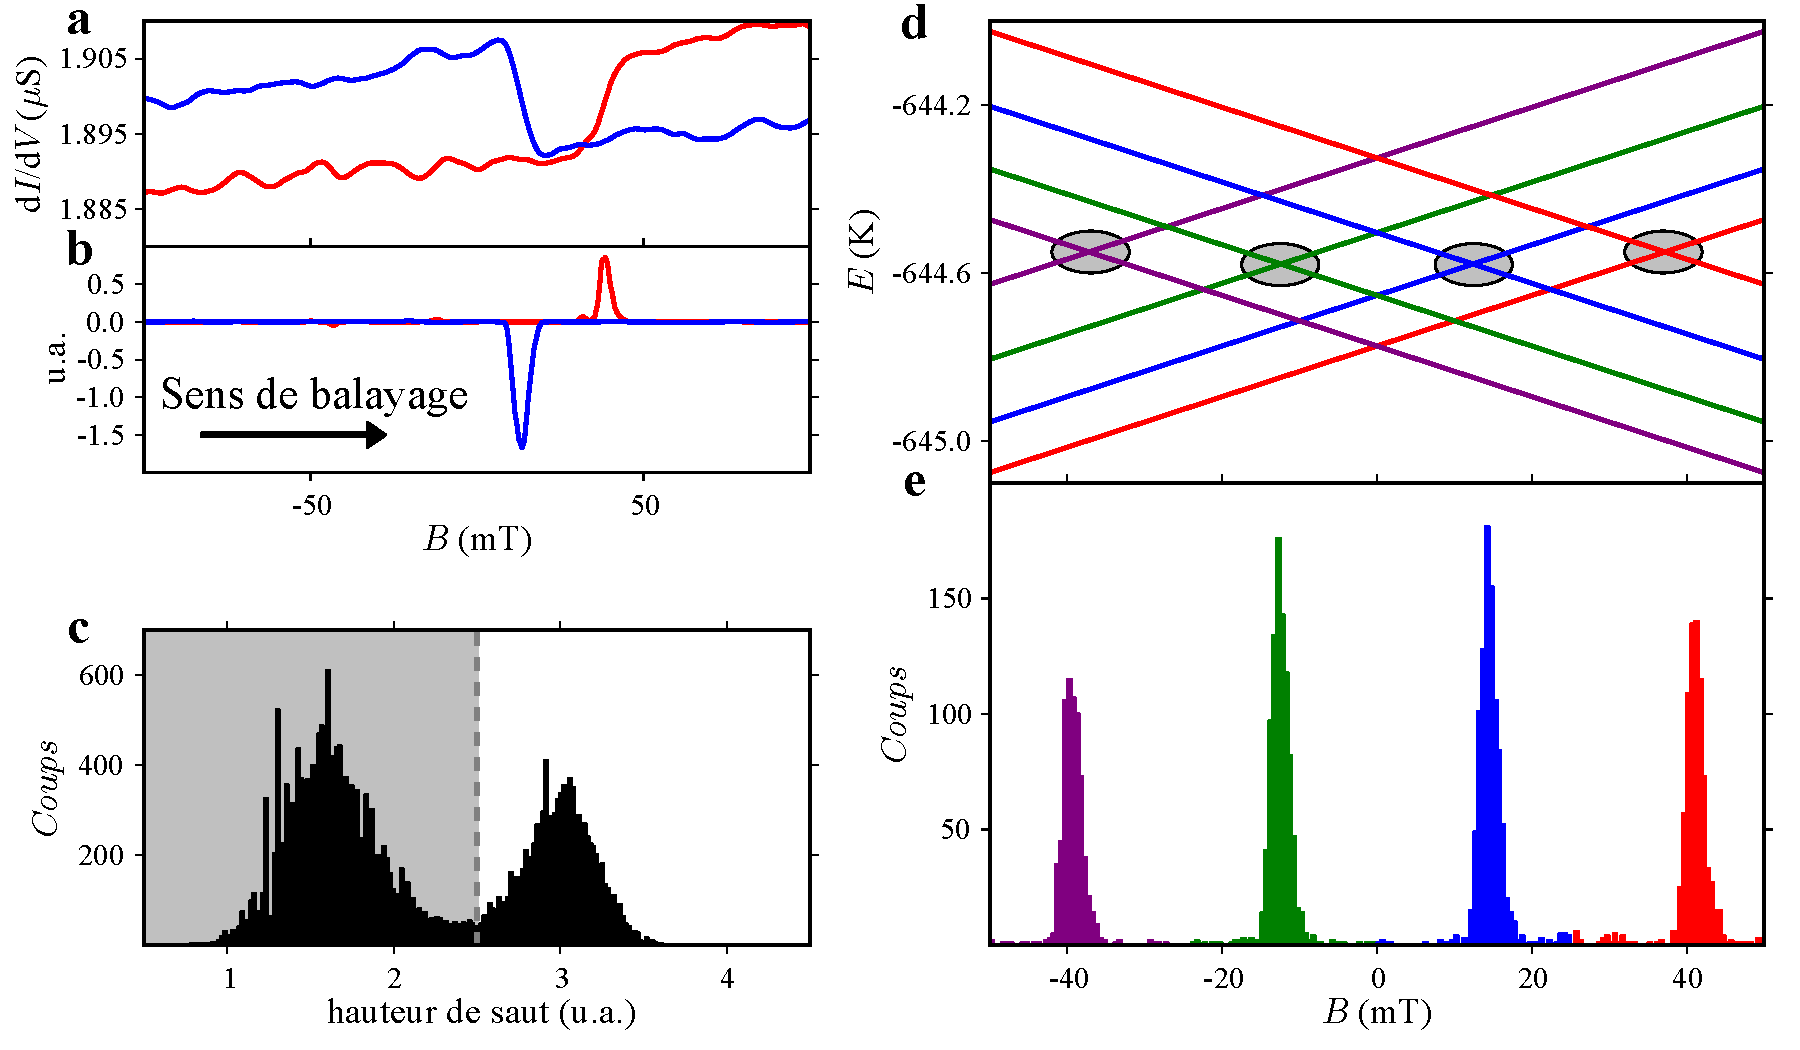
\includegraphics[scale=0.45]{Resultats/CondJump/CondJump.pdf} 
\caption{\textbf{a} - Mesure de deux sauts de conductance montrant deux variation $\Delta g$ de signes opposés. \textbf{b} - Signal correspondant à la mesure \textbf{a} filtrée : les sauts de conductance sont transformés en pics dont l'orientation (vers le haut ou vers le bas) dépend du signe de $\Delta g$. \textbf{c} - Statistique de la hauteur des sauts : cette dernière met en évidence deux distributions : celle contenue dans la zone grise correspond à de petites transitions relatives au bruit de mesure; la seconde distribution correspond au signal induit par le retournement de l'aimantation. \textbf{d} - Diagramme Zeeman de l'état fondamental de la molécule de TbPc$_2$ à faible champ : les anti-croisements donnant lieu au phénomène de QTM sont repérés par les cercles grisés. \textbf{e} - Statistique portant sur la position en champ des retournements de l'aimantation : quatre résonances sont clairement identifiables et correspondent aux quatre anti-croisements.}
\label{analyse_saut}
\end{figure}


\subsection{Méthode de détection}
La première étape de notre méthode de mesure est de détecter chaque saut en conductance, relatif à un retournement de l'aimantation. Une mesure type d'un saut de conductance est présenté dans la Fig.\ref{analyse_saut}.\textbf{b}. Il faut, dans un premier temps, rendre le signal plus facilement exploitable par l'application d'un filtre détaillé dans~\cite{Y.1995}. La Fig.\ref{analyse_saut}.\textbf{a} correspond au signal de la Fig.\ref{analyse_saut}.\textbf{b} après son application. Les sauts de conductances ont été convertis en pics, qu'il est facile d'extraire par une méthode des extrema. Le signe du saut de conductance est donné par l'orientation des pics : un changement positif correspond à un maximum; un changement négatif à un minimum.

Il faut ensuite procéder à l'analyse statistique de ces sauts. Pour cela, il est important de garder à l'esprit qu'il peut y avoir des mesures sans saut, le retournement étant un événement probabiliste. Dans ce cas, les extrema détectés ne correspondront pas à un signal véritable mais à un artefact. Pour ne prendre en compte que le signal, on effectue une statistique de la hauteur des pics du signal filtré. La Fig.\ref{analyse_signe_saut}.\textbf{d} présente le résultat d'une telle statistique pour 12000 mesures. Deux distributions sont clairement identifiables : une distribution avec de faibles sauts correspondant au bruit de mesure~(zone grisée); une distribution de sauts marqués correspondant à des retournements de l'aimantation. Cette statistique permet de fixer un seuil~(limite entre zone grisée et non grisée), et de filtrer les sauts détectés en conséquence.

A partir des sauts sélectionnés, on effectue une étude statistique des champs de retournement de l'aimantation. La Fig.\ref{analyse_saut}.\textbf{e} présente une telle statistique, effectuée sur 6000 mesures faites à faible champ. On peut facilement identifier quatre résonances, c'est à dire, quatre valeurs du champ pour lesquelles l'aimantation de la molécule a une forte probabilité de se retourner. 

En comparant cette mesure avec le diagramme Zeeman de la molécule de TbPc$_2$~(cf Fig.\ref{analyse_saut}.\textbf{c}), on peut associer chaque résonance à un des anti-croisements repérés par des cercles. Sachant que chacun d'eux correspond à une situation où le QTM est possible, on peut en déduire que la présence de ces résonances est la \textbf{mesure directe} du phénomène de QTM à l'échelle d'une seule molécule. 

De plus, chaque anti-croisement est associé à un unique état de spin nucléaire. La mesure de la position en champ magnétique du retournement de l'aimantation est donc une \textbf{mesure indirecte} de l'état de spin du noyau de terbium. C'est cette dernière propriété que nous utiliserons dans la suite pour étudier la dynamique du spin nucléaire.

\subsection{Interprétation physique de $\Delta g$}
Jusqu'à présent, nous n'avons pas utilisé le signe de $\Delta g$ comme élément d'analyse. Pourtant, dans le cadre de notre modèle, celui-ci donne accès à la nature de la transition : $J_z = \pm6 \rightarrow J_z = \mp 6$. Il existe une méthode expérimentale, basée sur la population thermique des spins nucléaires, permettant de vérifier notre hypothèse.

Supposons que l'on se place dans l'état initial $J_z=+6$ et $B<0$. Au regard du digramme Zeeman de la Fig.\ref{TbPc2Zeeman}.\textbf{d}, et du fait de la relaxation, l'état de spin $I_z = -3/2$ devrait être le plus probablement mesuré. L'inverse est vrai pour l'état initial $J_z=-6$ et $B<0$. La Fig.\ref{analyse_signe_saut} présente une étude statistique des champs de retournement en fonction du signe de $\Delta g$. Lorsque $\Delta g> 0$~($\Delta g< 0$), l'état de spin nucléaire le plus probable est l'état $I_z = -3/2$~($I_z = +3/2$), ce qui correspond à un état initial $J_z=+6$~($J_z=-6$). $\Delta g> 0$~($\Delta g< 0$) correspond donc à la transition $J_z = +6 \rightarrow J_z =  - 6$~($J_z = -6 \rightarrow J_z =  + 6$).

\begin{figure}
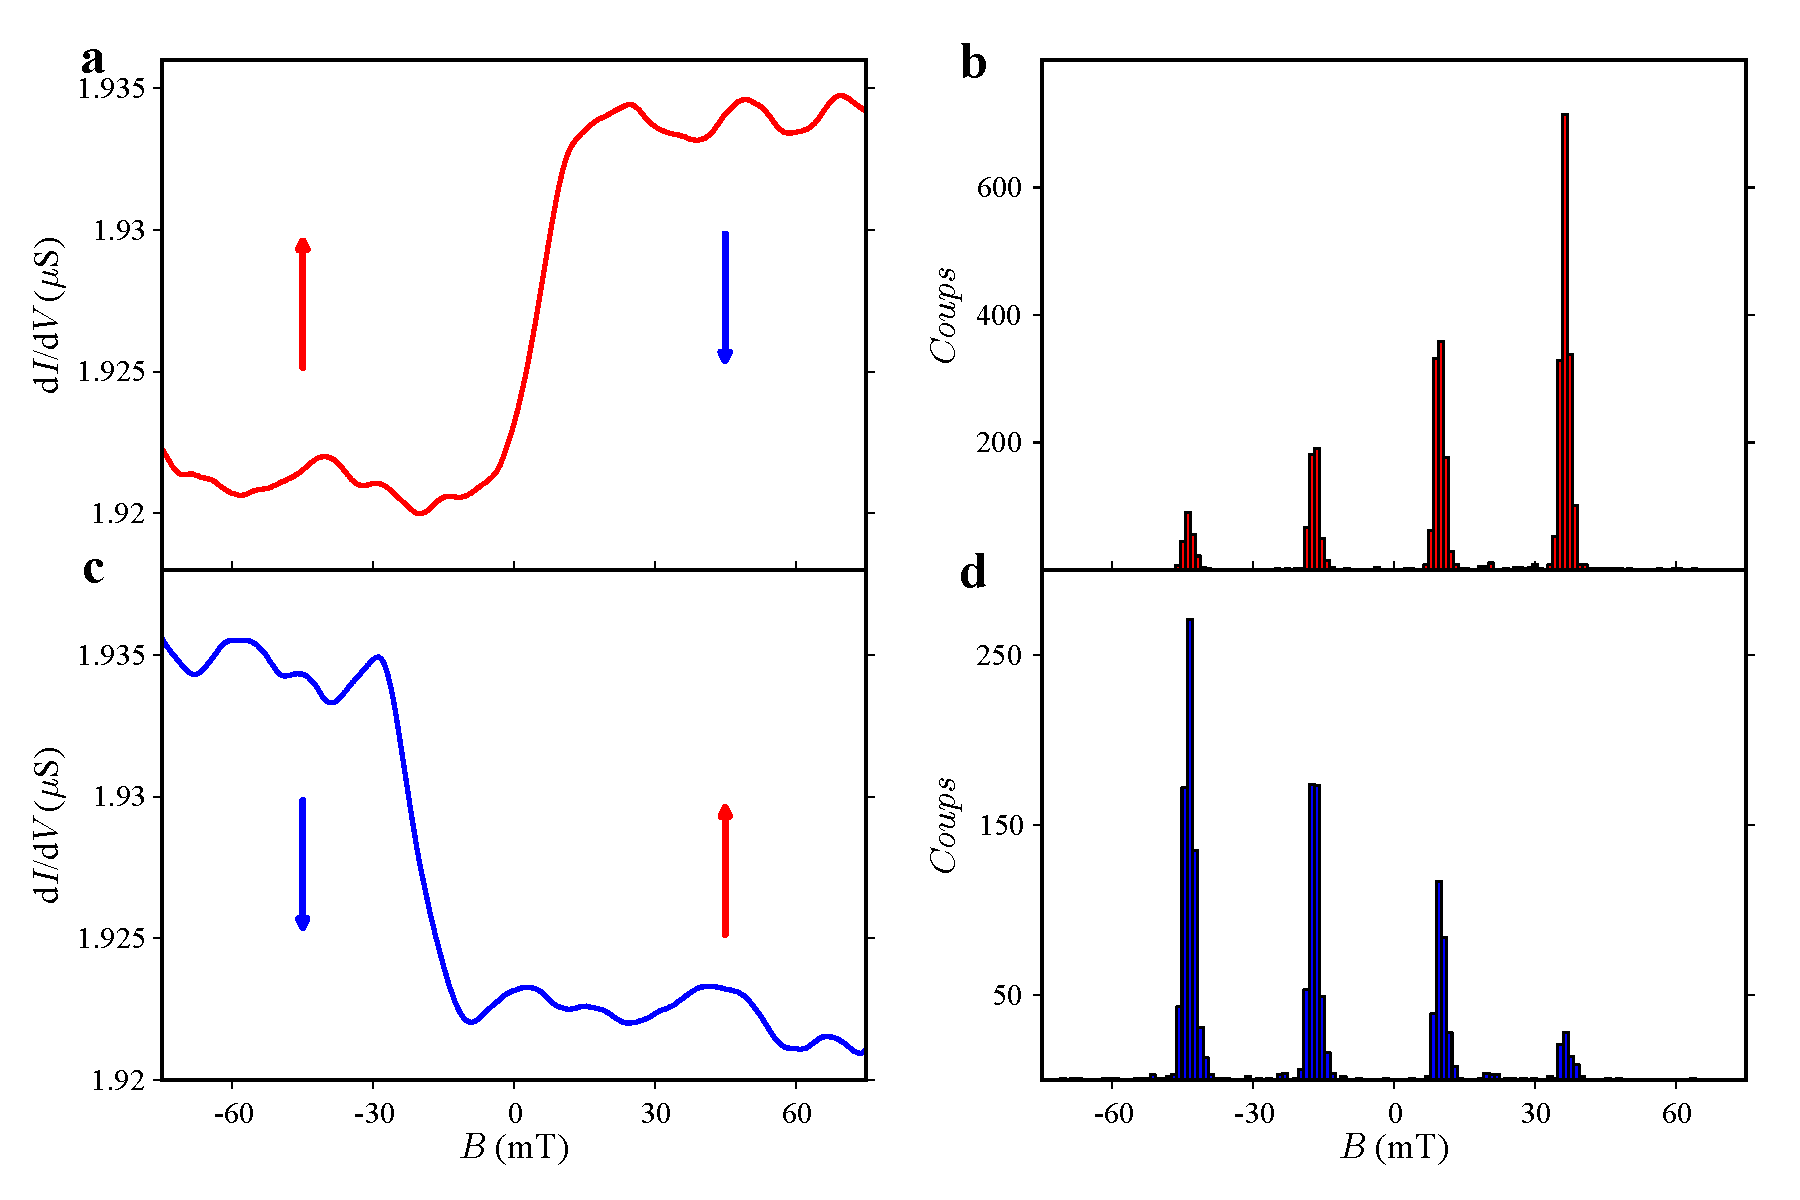
\includegraphics[scale=0.45]{Resultats/JumpSens/JumpSens.pdf} 
\caption{\textbf{a}(\textbf{c}) - Mesure d'un saut de conductance en fonction de l'état initial, la couleur de la courbe étant fonction de ce dernier. \textbf{c}(\textbf{d}) - Statistique des champs de retournement en fonction de l'état initial (signe de $\Delta g$) montrant clairement l'inversion de population des spins nucléaires. La couleur des histogrammes est donnée par l'état initial auxquels ils correspondent.}
\label{analyse_signe_saut}
\end{figure}

On peut donc affirmer de façon certaine, que la variation en conductance $\Delta g$ est directement liée au retournement de l'aimantation, et que son signe nous renseigne sur le sens de la transition.


\subsection{Choix du point de fonctionnement}
La zone où la variation de conductance est la plus sensible au potentiel chimique, se situe au niveau des points de dégénérescence. En effet, dans cette zone, la moindre variation du potentiel chimique entraîne une forte variation en courant. C'est donc dans cette zone, que l'on va logiquement se placer afin d'obtenir une sensibilité maximale. Dans un système idéal, on a $\frac{\partial g}{\partial \mu}_{\text{d}} = -\frac{\partial g}{\partial \mu}_{\text{g}}$, où $d$ et $g$ signifient à droite et à gauche du point de dégénérescence. Ceci a notamment été mis en évidence par~\cite{Datta2011} dans le cadre de nanoparticules magnétiques couplées par effet magnéto-Coulomb à un nanotube.

\begin{figure}
\parbox{7cm}{
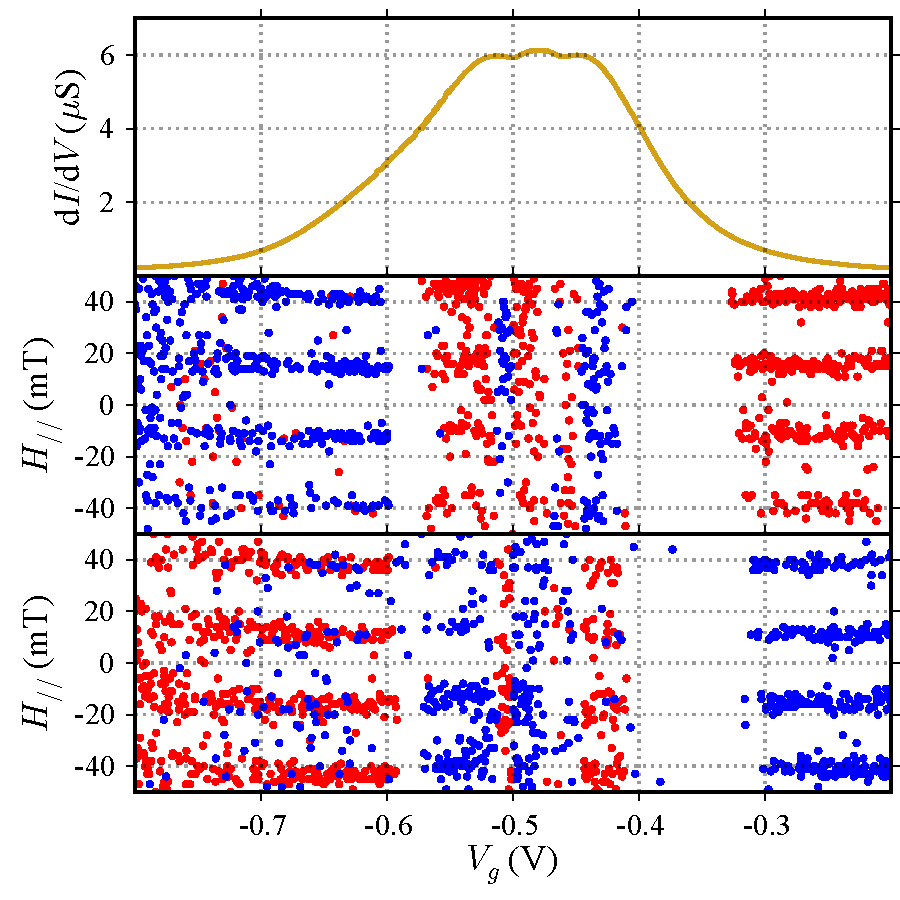
\includegraphics[scale=0.45]{Resultats/PointFonct/PointFonct.pdf} 
}
\parbox{6.5cm}{\caption{\textbf{Panel haut} - Mesure de la conductance différentielle en fonction de la tension de grille $V_g$ à tension source-drain nulle. \textbf{Panel du milieu~(bas)} - Mesure du signe de $\Delta g$ en fonction de la tension de grille $V_g$ et du champ transverse $H_{//}$ durant la trace~(retrace) : les points rouges correspondent à $\Delta g >0$; les points bleus à $\Delta g <0$. Les zones blanches dénotent des valeurs de tension de grille pour lesquelles le signal magnétique n'est pas résolu.}
\label{point_fonctio}
}
\end{figure}

Dans notre système, cette propriété n'est pas respectée et le résultat obtenu est plus complexe. La Fig.\ref{point_fonctio} montre le signe du changement de conductance correspondant à un retournement, en fonction de la tension de grille $V_g$. On observe trois type de zones : les zones où le signal est trop faible pour être détecté; des zones où le bruit généré par les phénomènes de transport masque le signal magnétique.; enfin des zones où le signal magnétique est net et les résonances clairement visibles. Dans ces dernières, on observe des transitions d'un signe à l'autre similaire à un changement de signe de $\frac{\partial g}{\partial \mu}$. Notre système est en cela relativement éloigné du système idéal que nous avons utilisé jusqu'à maintenant. L'origine des zones de transitions ne nous apparaît toujours pas claire. En revanche, lorsque l'on s'éloigne des zones à forte conductance, le système se comporte de la manière attendu, avec un changement dans le signe $\frac{\partial g}{\partial \mu}$, de part et d'autre du point de dégénérescence.

Dans la suite, nous nous placerons loin des zones de transition, afin d'éviter toute mauvaise interprétation dans le signe de $\Delta g$.


\subsection{Procédure d'alignement}

L'une des caractéristiques principales d'un aimant moléculaire est de posséder un axe facile, c'est à dire, un axe le long duquel le moment magnétique "préfère" s'aligner. C'est suivant cet axe que le champ magnétique nécessaire au retournement de l'aimantation est le plus faible. Pour cette raison, il est indispensable de l'identifier de façon à minimiser le champ magnétique à appliquer à l'échantillon. Dans le cas d'un mauvais alignement, seule la projection du champ magnétique appliqué suivant l'axe facile,  contribue au retournement. Dans le cas extrême où le champ appliqué serait perpendiculaire à cet axe, aucun retournement ne pourrait être observé.

Expérimentalement, la présence d'un retournement peut se mesurer à travers la présence d'un hystérésis dans la mesure de conductance. Celui-ci apparaît lorsque l'on balaie le champ magnétique des valeurs négatives aux valeurs positives et inversement, tout en mesurant la conductance du système. La Fig.\ref{alignement}.\textbf{b} met en évidence cet hystérésis. Une lecture plus claire peut être obtenue en soustrayant l'aller au retour comme le montre la Fig.\ref{alignement}.a. En effectuant cette mesure pour différents angles de champ magnétique, on obtient la mesure de la Fig.\ref{alignement}.\textbf{c}. Celle-ci met en évidence un "axe facile" le long duquel le retournement se fait à faible champ, et un axe difficile le long duquel le champ n'est pas suffisant pour observer de retournement.

\begin{figure}
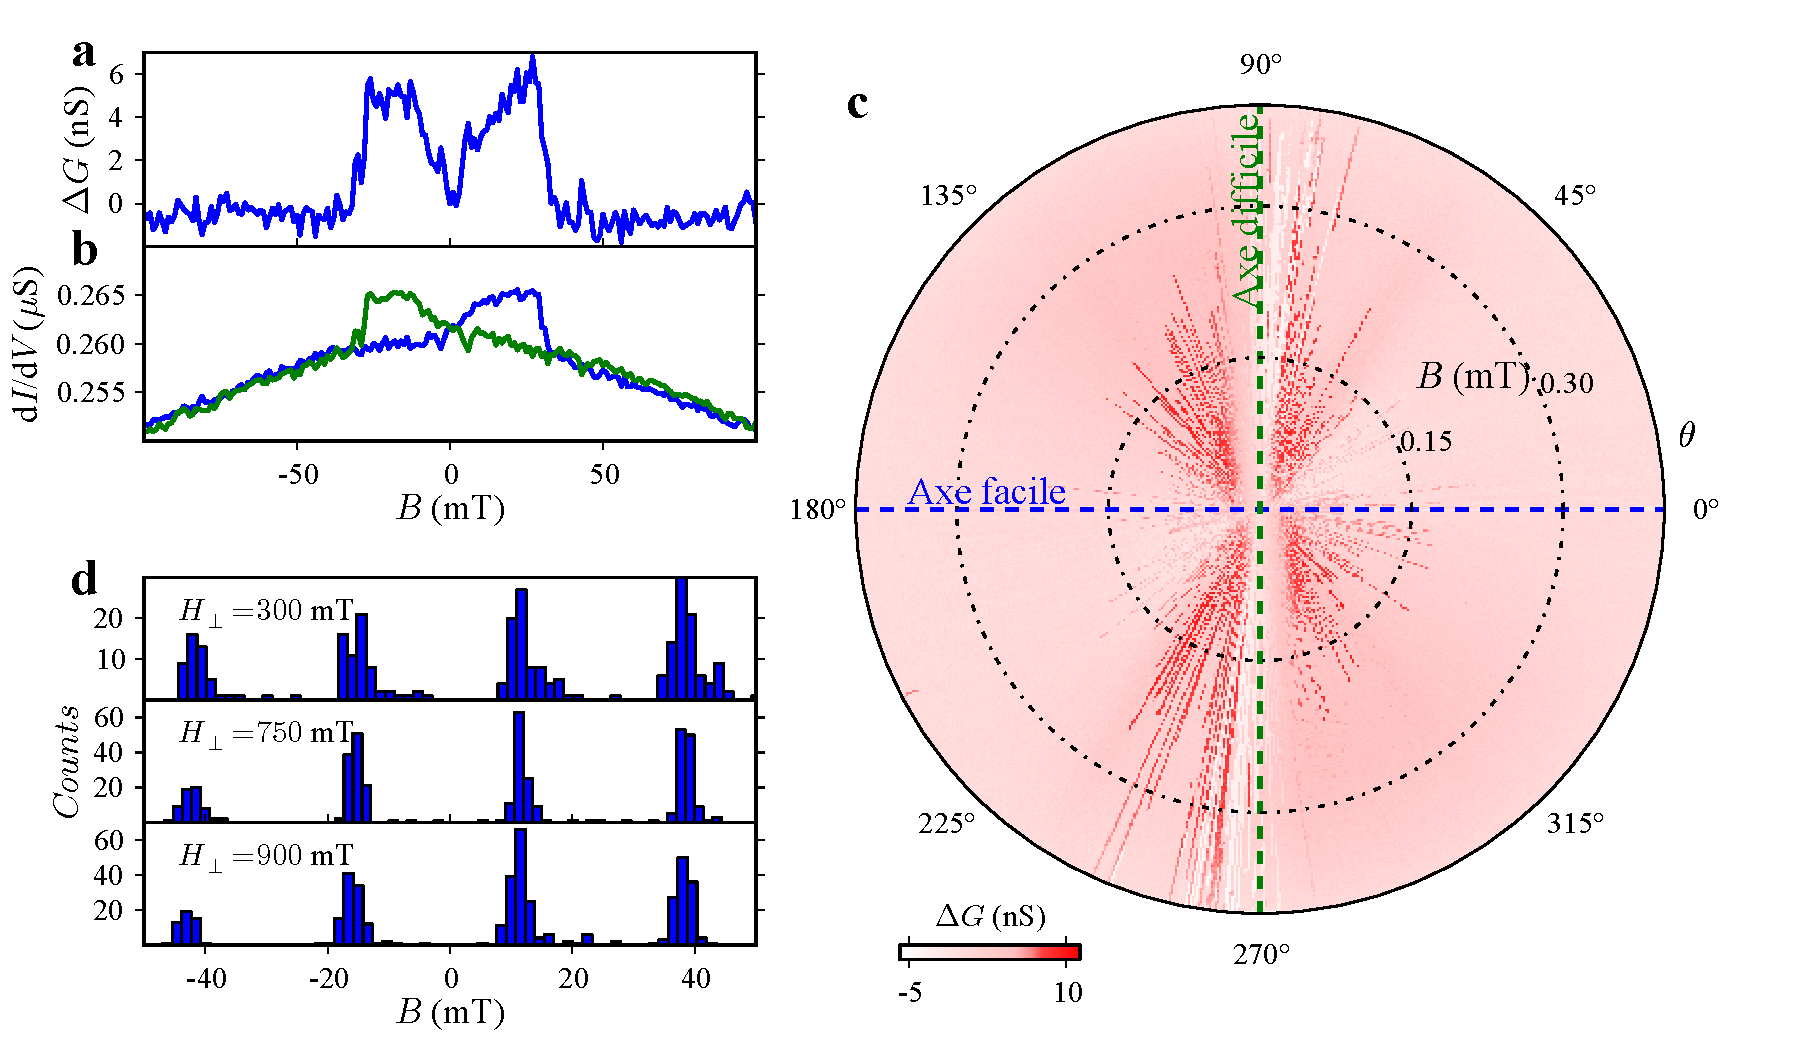
\includegraphics[scale=0.45]{Resultats/Alignement/Alignement.pdf} 
\caption{\textbf{a}~-~Mesure de l’hystérésis en conductance en fonction du champ magnétique entre la trace et la retrace obtenu à partir de mesure de \textbf{b}. \textbf{b}~-~Mesure de la conductance en fonction du champ magnétique pour la trace~(en vert) et la retrace~(en rouge). \textbf{c}~-~Mesure de l'hytérésis en fonction de l'angle $\theta$. Les axes facile (retournement à faible champ) et difficile (retournement impossible) sont clairement identifiable. \textbf{d}~-~Mesure de la position des résonance en champ magnétique parallèle en fonction du champ transverse. La position des résonance reste identique montrant le bon alignement de nos axes}
\label{alignement}
\end{figure}

Cependant, il faut garder à l'esprit que ``l'axe facile" identifié sur cette figure, n'est en fait que la projection de celui-ci dans le plan défini par la mesure. Pour s'aligner, il est donc préférable d'identifier deux vecteurs du plan difficile. A cette fin, on effectue une deuxième mesure dans un plan différent, afin d'obtenir un deuxième axe difficile, et ainsi pouvoir définir le plan difficile. Sachant que l'axe facile est orthonormal à celui-ci, un produit vectoriel de deux vecteurs appartenant au plan difficile nous donne l'axe facile. Expérimentalement, l'angle $\theta$ permettant d'obtenir la Fig.\ref{alignement}.\textbf{c} est défini à l'aide de deux bobines. L'angle $\phi$ nous permettant de faire la mesure dans deux plans différents est, quant à lui, obtenu par rotation de la dilution le long de l'axe d'une des bobines.


Afin de vérifier le bon alignement de nos axes magnétiques, nous avons mesuré la position des résonances à faible champ en fonction d'un champ que l'on applique dans le plan difficile, et que l'on appellera dans la suite champ transverse. Si l'alignement est correct, la projection d'un tel champ sur l'axe facile est nulle. La position des résonances ne devrait donc pas varier. La Fig.\ref{alignement}.d présente la position de ces résonances pour trois champs transverses, et confirme le bon alignement de nos axes magnétiques, avec l'axe facile de la molécule.

\section{Magnétisme électronique}
Avant de nous intéresser au magnétisme nucléaire de notre système, nous allons nous attarder un instant sur le magnétisme électronique. Nous verrons tout d'abord comment on peut reconstituer le cycle d'hystérésis d'une molécule unique. On décrira notamment l'influence de l'environnement sur ce dernier, et nous montrerons le rôle important que peut jouer le champ transverse dans la diminution de ces interactions à faible champ. Nous verrons enfin que ce dernier peut également rendre l'extraction des données plus aisée.

\subsection{Reconstruction du cycle d’hystérésis}
Dans notre expérience, nous n'avons accès qu'à un seul aimant moléculaire. Il nous faut donc utiliser l'hypothèse ergodique à savoir : mesurer un assemblé de $N$ molécules identique, est équivalent à mesurer $N$ fois la même molécule. Pour le reste, la méthode de mesure est identique à celle employé avec la technique microSQUID. L'aimantation est amenée à saturation, ce qui revient, dans notre cas, à appliquer un champ magnétique suffisamment grand pour que l'aimantation de la molécule se retourne. Le champ magnétique est ensuite balayé et la position en champ magnétique du retournement de l'aimantation est relevée. Ce cycle est effectué $N$ fois afin de pouvoir constituer une statistique~(dans nos expérience, $N$ à pris des valeur entre 1000 et 22000 selon les cas). L'histogramme correspondant est présenté dans la Fig.\ref{CompAimant}.\textbf{b} dans le cas de 800 aller-retour en champ magnétique. A partir de ce dernier, on peut ensuite reconstruire l'hystérésis de l'aimantation. Pour cela on note $\mathscr{N}(B)$ le nombre de molécules s'étant retournées avant le champ magnétique $B$ et on attribue le moment magnétique $\frac{M_s}{N}$ à chaque molécule, $M_s$ étant l'aimantation de saturation et $N$ le nombre total de mesures. L'aimantation en fonction du champ magnétique prend alors la forme suivante :
\begin{eqnarray}
M(B) =\pm \frac{M_s}{N}(2\mathscr{N}(B) -1)\nonumber
\end{eqnarray}

Le signe est déterminé par celui du champ de saturation initial : positif pou un champ de saturation négatif; négatif pour un champ de saturation positif. Pour une comparaison plus aisée avec les mesure micro-SQUID, on peut ré-exprimer la formule précédente comme suit :
\begin{eqnarray}
\frac{M}{M_s}(B) =\pm \frac{1}{N} (2\mathscr{N}(B) -1)
\end{eqnarray}


Le résultat obtenue pour un champ de saturation de $\pm 400 \, mT$, une vitesse de balyage de $50\,mT.s^{-1}$, un champ transverse de $750\,mT$ et pour $N$ mesures, est présentée dans les Fig.\ref{CompAimant}.\textbf{b}. Afin de faciliter l'analyse de la mesure, j'ai choisi la de diviser en deux zones : champ faible pour $|B|< 100\,mT$, champ fort pour $|B|>100\,mT$.

\begin{figure}
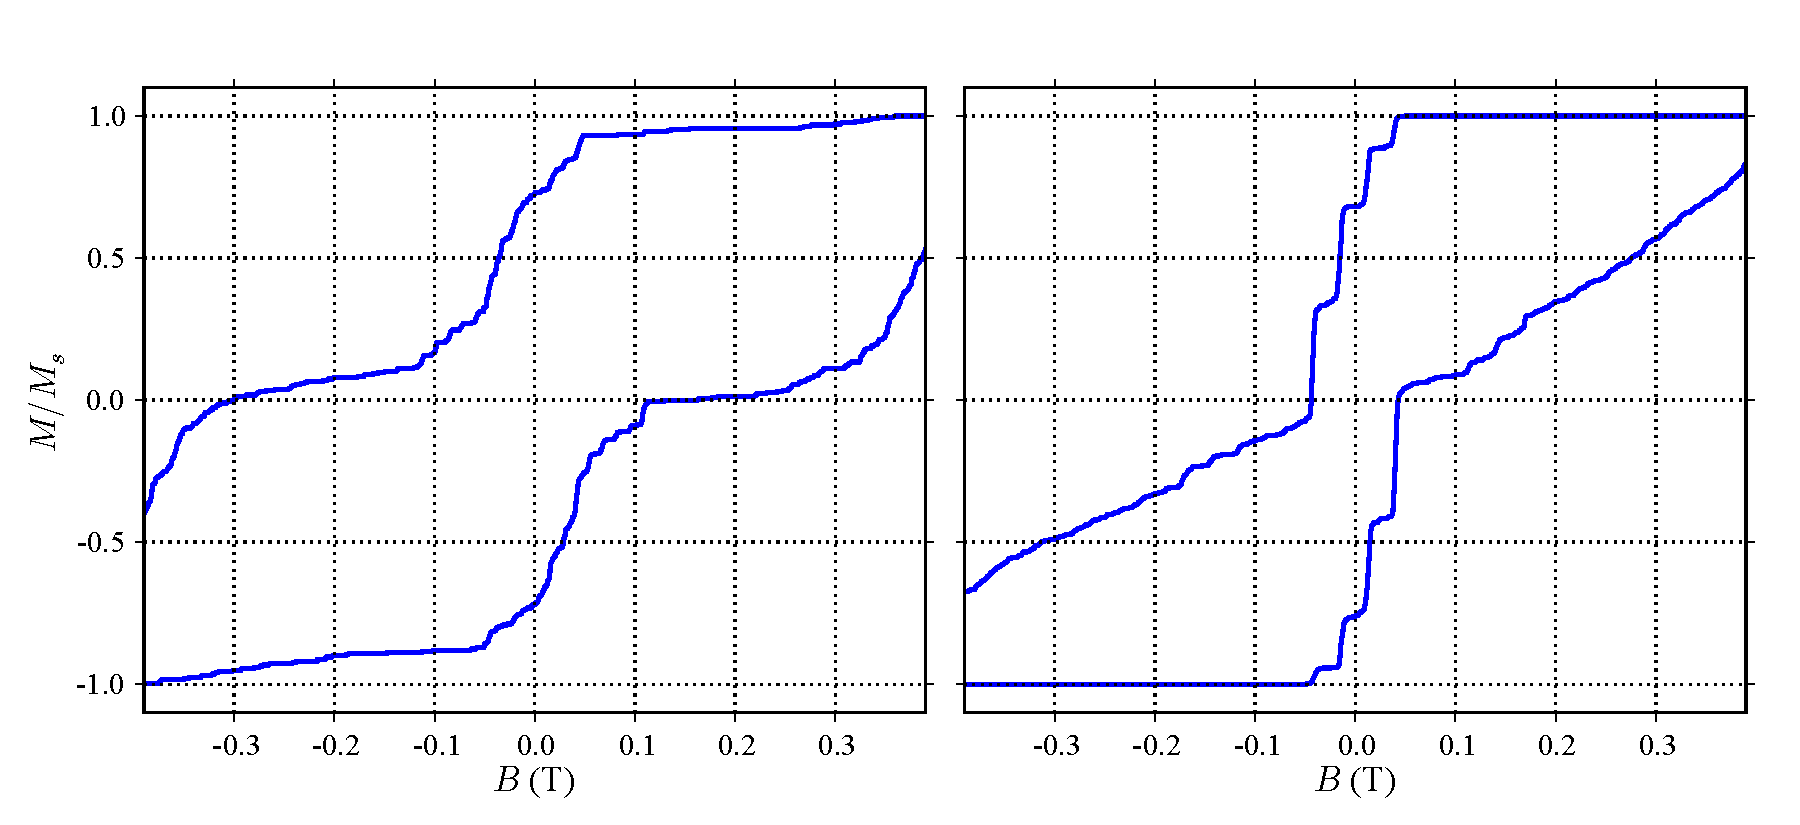
\includegraphics[scale=0.45]{Resultats/CompCrisMolUnique/CompCrisMolUnique.pdf} 
\caption{Hysteresis de la molécule TbPc$_2$ reconstruit à partir des mesures en transports sans champ transverse~(\textbf{a}), et avec un champ transverse de $750\,mT$~(\textbf{b}).}
\label{CompAimant}
\end{figure}

A faible champ, la structure en marche, correspondant au quatre anti-croisements de la Fig.\ref{TbPc2Zeeman}.\textbf{d} et caractéristique du phénomène de QTM~\cite{Thomas1996,Friedman1996} est clairement visible. Il est à noté que, dans le cas de la mesure obtenues à partir d'un cristal moléculaire, un nombre plus élevés de marches est mesuré. Ces dernières sont très certainement induites par des interactions entre les différents centres magnétique du cristal~\cite{Wernsdorfer2002}, et ce, malgré la dilution à 10\%.

A champ fort là encore, il subsiste quelques différences entre la mesure microSQUID et celle obtenue avec notre système. Alors que dans le cas d'un cristal moléculaire le retournement assisté par le bain de phonons est le seul mécanisme impliqué, la présence  de marches supperposé à un retournement continue est clairement visible dans le cas de notre système. Ne disposant pas, pour le moment, de modèle satisfaisant expliquant ces caractéristiques, nous ne nous attarderons pas sur cette dernière partie du cycle d’hystérésis et nous de développerons une analyse détaillée que de la zone champ faible.

\subsection{Le r\^ole du champ transverse}

La mesure de la Fig.\ref{CompAimant}.\textbf{b} a été réalisée pour un champ transverse de $750mT$. La présence de ce champ transverse n'est pas anodine, mais au contraire, nécessaire à l'obtention d'une mesure faiblement perturbé par l'environnement. En fait, la présence d'un champ transverse à deux conséquence : l'une physique puisqu'il réduit les perturbations du système, et l'autre de l'ordre de la mise en oeuvre de la détection. Nous allons détailler ces deux points.

\subsubsection{Conséquences physiques}
Notre aimant moléculaire, lorsqu'il est piégé dans notre interstice nanométrique, n'est pas à proprement parlé isolé. Il peut subir l'influence d'une autre molécule, d'une impureté magnétique piégée dans l'oxyde de grille, ou tout autre système susceptible d'échanger de l'énergie. Cependant, il est possible d'isoler notre aimant moléculaire de façon artificielle, par l'application d'un fort champ transverse. Ce dernier venir aligner les systèmes magnétiques environnant, ne leur laissant plus la possibilité d'interagir avec l'aimant moléculaire. Les propriétés magnétique de ce dernier sont, en revanche, peu perturbées par la présence de ce champ transverse.

L'amélioration dans la qualité de la mesure peut être apprécié en comparant un cycle d'hystérésis reconstitué à partir d'une mesure sans champ transverse~(cf Fig.\ref{TransInfl}.\textbf{a}), et la même mesure réalisé avec un champ transverse de $750\,mT$~(cf Fig.\ref{TransInfl}.\textbf{b}). Dans le premier cas, une multitude de marche à faible champ sont visible, et rendre compte des couplages multiples entre l'aimant moléculaire et son environnement. Dans le second cas, à faible champ, on identifie clairement les marches relatives au QTM. A plus fort champ, on constate encore la présence de marches secondaires, réminiscent du couplage à l'environnement, initialement présent à faible champ.

Dans la suite, l'ensemble des mesures a été fait avec un champ transverse de $750mT$.

\subsubsection{Impact sur la mise en œuvre}

La présence d'un champ transverse a également une conséquence sur la mise en oeuvre de la détection. Comme nous l'avons présenté dans la partie consacré à la technique de détection, il est nécessaire, pour mesurer le retournement de l'aimantation de façon efficace, de se placer sur un point tel que $\frac{\partial g}{\partial B} = cst$. Or, à faible champ, cette relation n'est plus vérifié et l'on observe un changement de signe de $\frac{\partial g}{\partial B}$  comme le montre la Fig.\ref{analyse_interaction}.\textbf{a}, ce qui n'est pas sans posé de problème. D'autant plus que le phénomène de QTM se déroule également à champ faible.

Nous avons observé, pour notre échantillon, une légère anisotropie de la conductance en fonction du champ magnétique. Cela se traduit, lorsque l'on applique un champ transverse, par un décalage de la zone d'inversion de signe de $\frac{\partial g}{\partial B}$, comme le montre la Fig.\ref{TransInfl}. On peut donc opérer des mesures avec un signe de  $\frac{\partial g}{\partial B}$ constant sur la totalité de la plage de champ magnétique nécessaire à la mesure.


\begin{figure}
\parbox{7cm}{
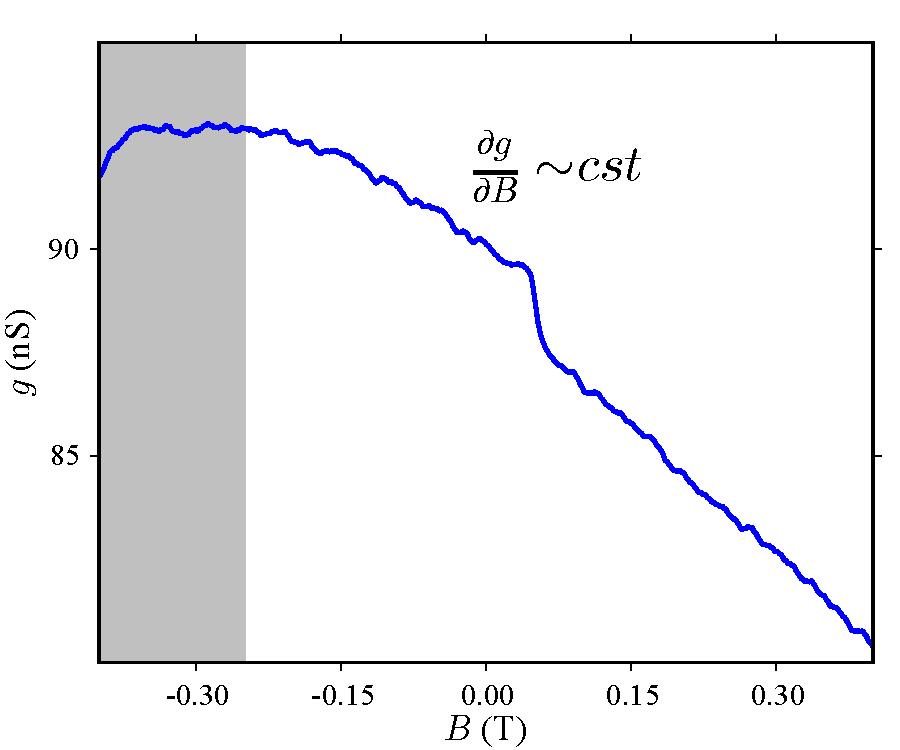
\includegraphics[scale=0.45]{Resultats/TransInfl/TransInfl.pdf} 
}
\parbox{6.5cm}{\caption{Mesure de la conductance différentielle $g$ pour un champ transverse $750mT$. La zone correspondant à $\frac{\partial g}{\partial B} \sim cst$ s'étant sur toute la zone de mesure.}
\label{TransInfl}
}
\end{figure}




Cette propriété a le mérite de faciliter considérablement l'interprétation du signe de $\Delta g$, et améliore grandement la capacité de détection à faible champ magnétique.

\section{Dynamique du spin nucléaire}


\subsection{Temps de relaxation}
Le spin nucléaire, du fait de son couplage relativement faible à l'environement, possède généralement un temps de vie élevé. Afin de pouvoir vérifier cette propriété, il nous faut pouvoir mesurer l'évolution des états du spin nucléaire en fonction du temps. Nous avons choisi pour cela une technique simple consistant à mesurer l'état du spin nucléaire lors de deux mesures, en faisant varier le temps séparant ces dernières. Du fait de l'aspect chronophage de cette procédure~(jusqu'à plusieurs jours par mesure), nous avons choisi cinq temps d'attente différents : $0,5,10,20$ et $50$ secondes. Pour chacune de ces valeurs, $22000$ balayges ont été effectués afin d'obtenir une statistique significative.


\begin{figure}
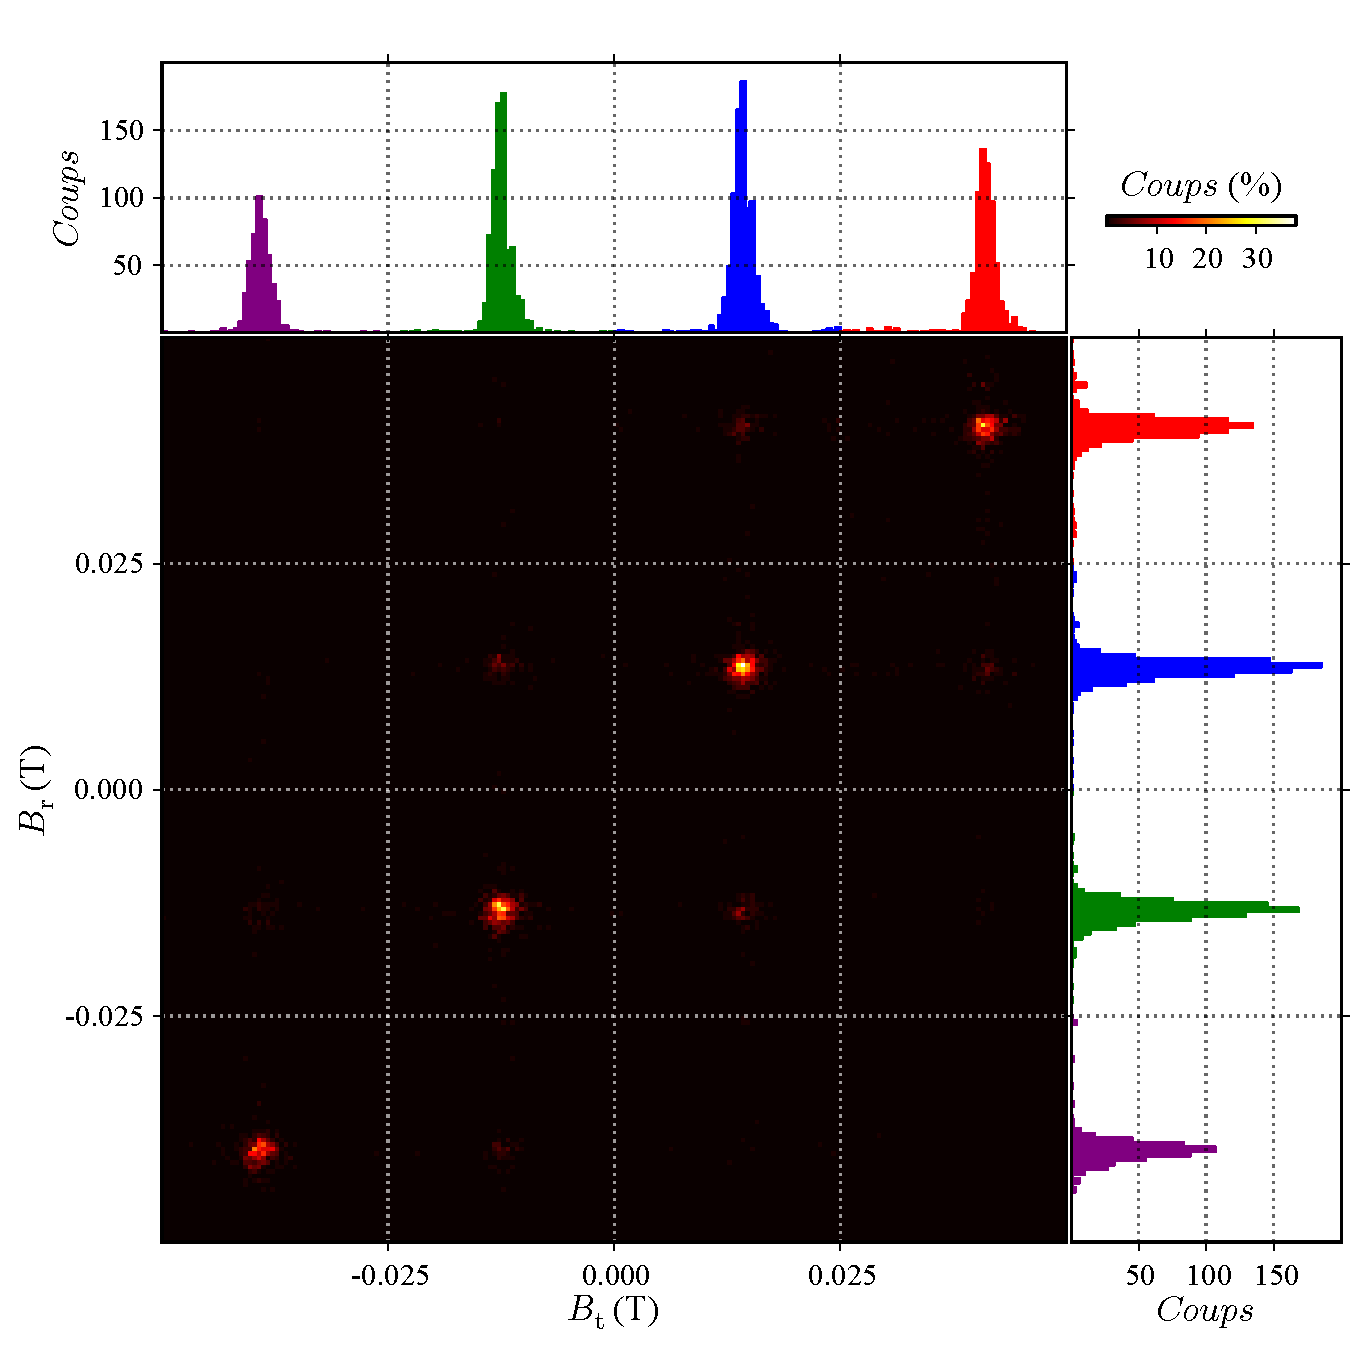
\includegraphics[scale=0.45]{Resultats/Hist2D/Hist2D.pdf} 
\caption{La cartographie couleur en deux dimensions représente l’histogramme de corrélation entre la position en champ magnétique des retournements ayant lieu durant la trace et la retrace.Celui-ci a été obtenu à partir de 22000 traces et retraces mesurées consécutivement et sans temps d'attente. Les histogramme à une dimension disposé le long des axes x et y représente respectivement les positions en champ magnétique des retournement durant la trace et la retrace. La prépondérance des éléments diagonaux atteste de la préservation de l'état de spin entre deux mesures.}
\label{correlations}
\end{figure}

L'évolution des états du spin nucléaire est représenté à l'aide d'un histogramme à deux dimensions. Le champ de retournement de la première mesure est repéré en abscisse et celui mesuré lors de la seconde mesure est représentée en ordonnée. Dans une telle représentation, les éléments diagonaux rendent compte d'un état de spin nucléaire qui ne change pas entre les deux mesures. Les éléments hors-diagonaux représente quant à eux las cas où l'état de spin nucléaire varie de $\Delta m_z^I = \pm 1,2,3$ où $m_z^I$ est la projection du moment angulaire du spin nucléaire sur l'axe $z$. La Fig.\ref{correlations} présente une telle mesure pour un temps d'attente nul. Pour faciliter la lecture, l'histogramme des champs de retournement de la première et deuxième mesures a été ajouté.

La Fig.\ref{evolution_temps} montre l'évolution de l'histogramme en fonction du temps d'attente entre les deux mesures. Les éléments diagonaux dominent jusqu'à un temps d'attente de $20$ secondes, prouvant que le spin nucléaire demeure majoritairement inchangé sur ce laps de temps. En revanche, pour un temps d'attente de $50$ secondes, on constate que les éléments diagonaux ne sont plus prépondérant signifiant le perte de l'état nucléaire entre les deux mesures. De plus, la résonance correspondant à l'état de spin $|-3/2 \rangle$ domine largement. Cela traduit la tendance du système à évoluer vers l'équilibre thermodynamique lorsque le temps d'attente devient trop élevé. Nus reviendrons sur ce dernier point dans la suite.

\begin{figure}[h!]
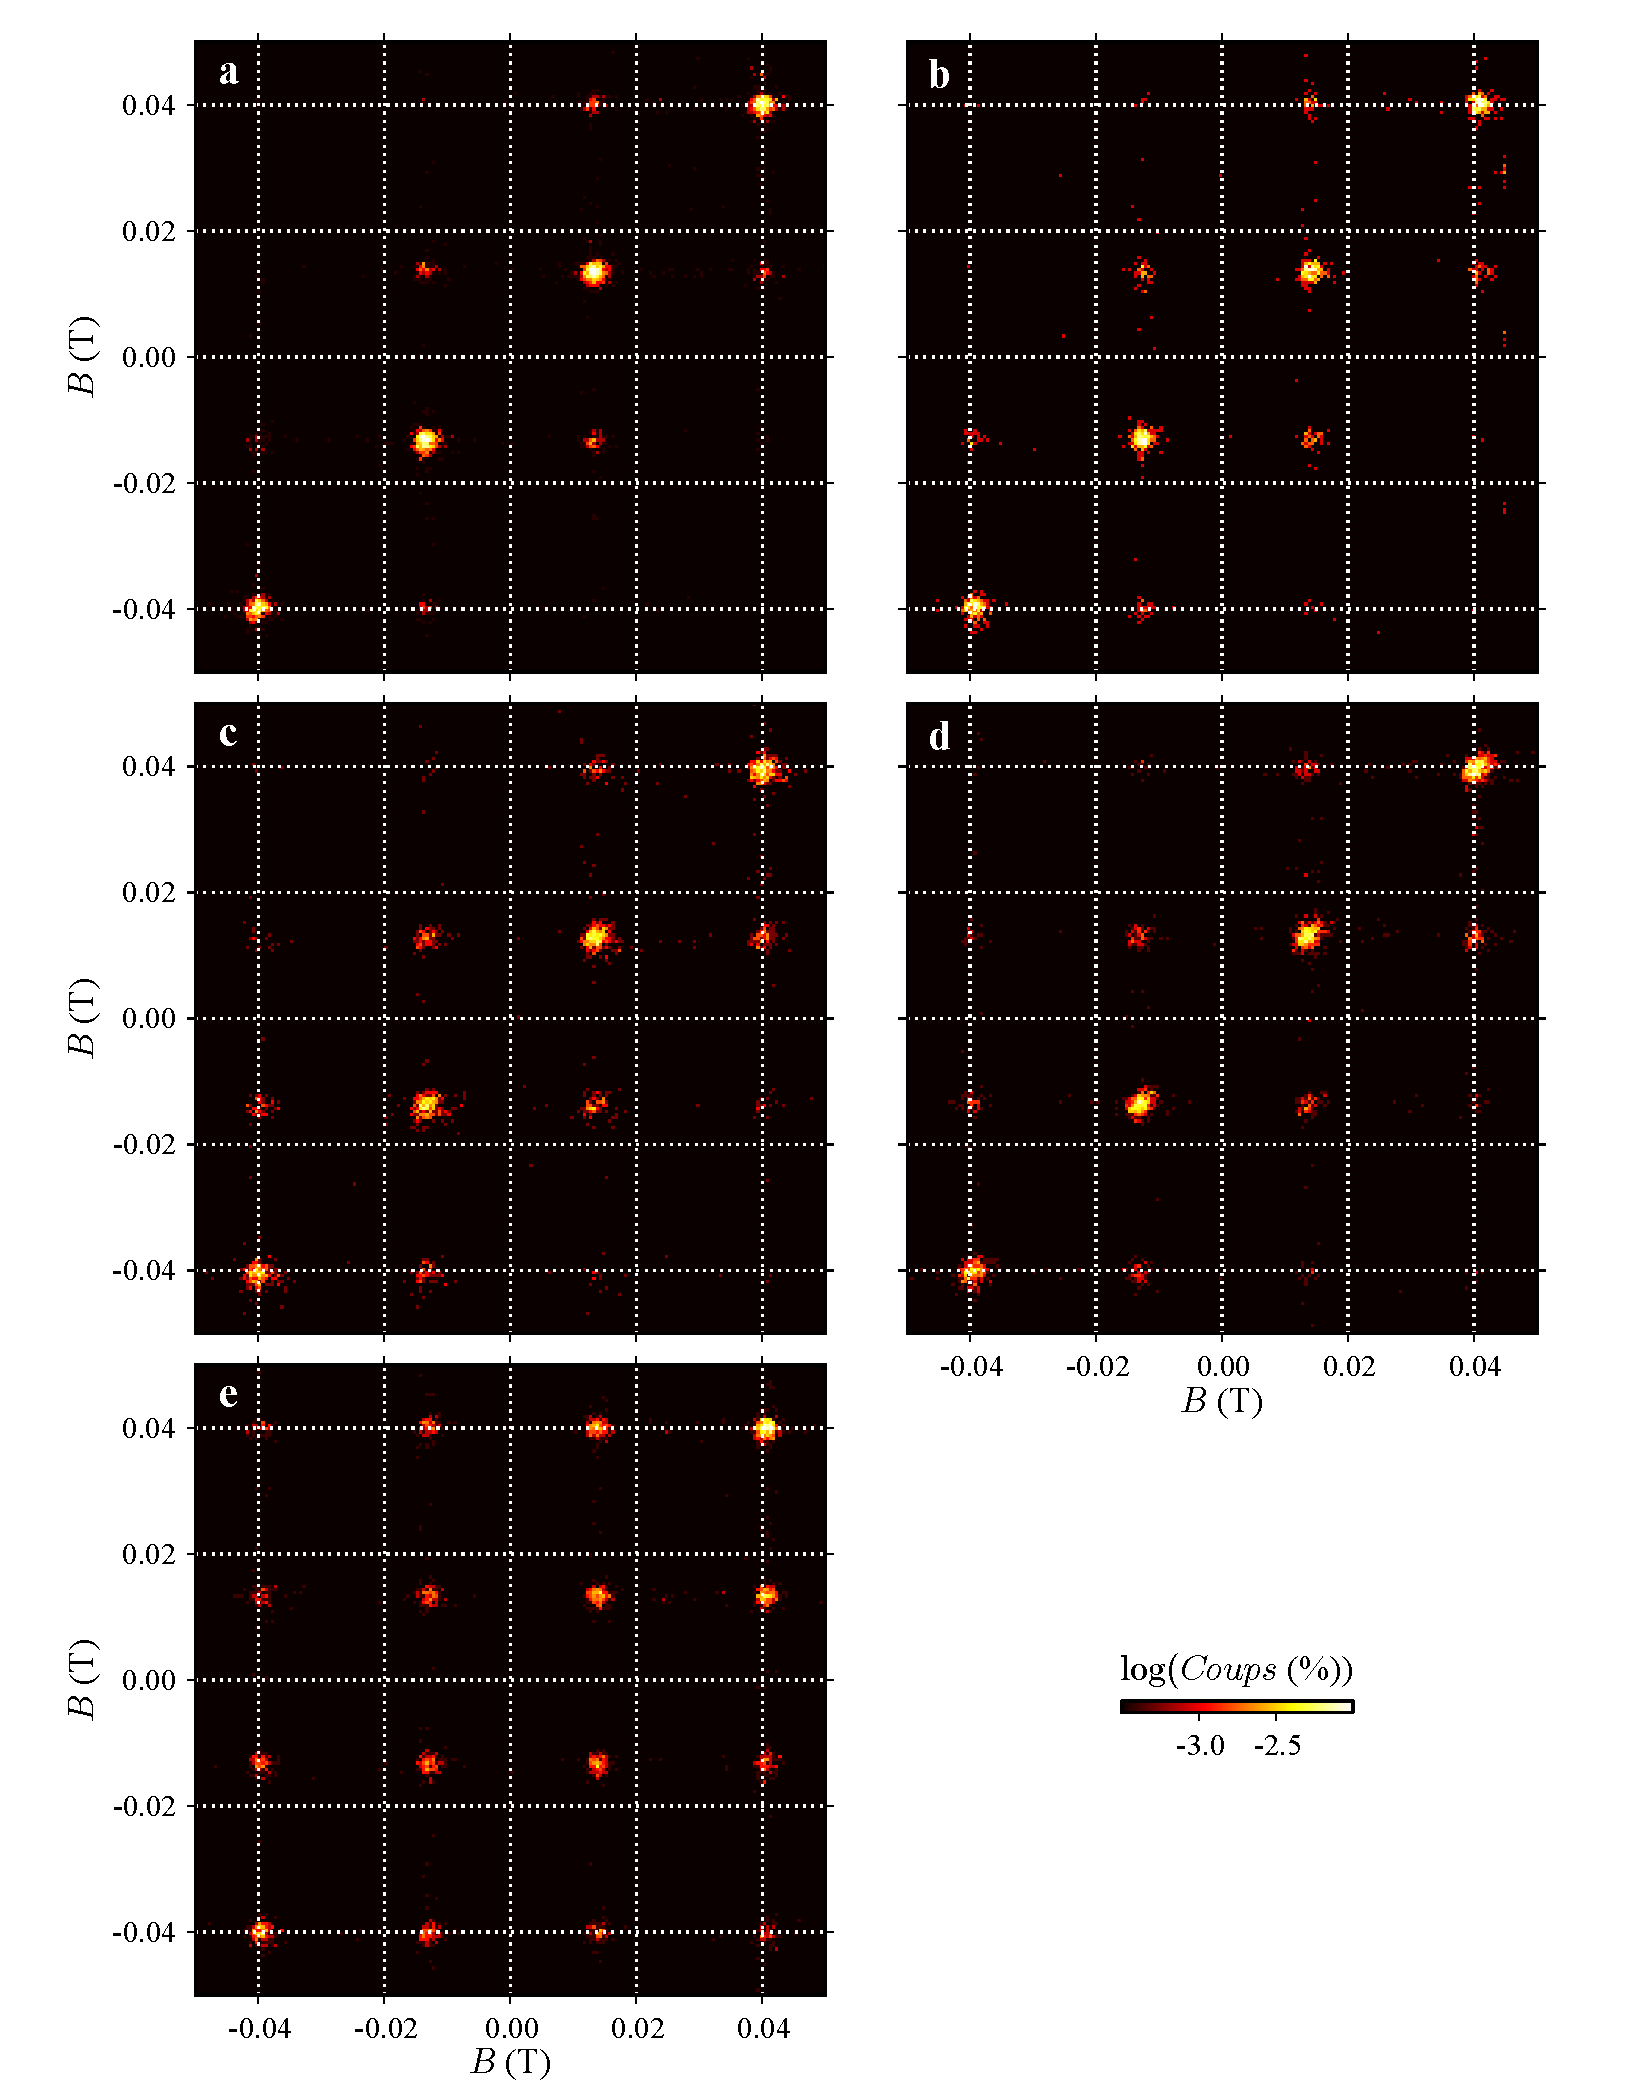
\includegraphics[scale=0.45]{Resultats/HistTime/HistTime.pdf} 
\caption{La cartographie a (b, c, d et e) présente un histogramme 2D rendant compte de la corrélation entre deux mesures obtenues durant la trace et la retrace, ces dernières étant séparé d'un temps d'attente de 0 secondes (5, 10, 20 et 50 secondes). La prédominance des élements diagonnaux pour des temps d'attente allant au-delà de la dizaine de seconde démontre le long temps de vie des états du spin nucléaire.}
\label{evolution_temps}
\end{figure}

\subsection{Perturbations induites par la mesure}
De m\^eme que nous pouvons étudier l'influence du temps d'attente sur le spin nucléaire, il peut \^etre intéressant d'évaluer l'influence de la mesure sur l'état de spin nucléaire. Pour cela, nous avons choisi d'utiliser la méthode présenté précédemment, en observant non plus l'évolution de l'état nucléaire en fonction du temps mais en fonction du nombre de mesures. Nous avons utilisé les donnée collecté sur 22000 balayages (11000 trace et autant de retrace) effectué sans temps d'attente.

La Fig.\ref{evolution_mesures} présente cette évolution après deux~(\textbf{a}), trois~(\textbf{b}), quatre~(\textbf{c}), cinq~(\textbf{d}) et six~(\textbf{e}) mesures. On constate qu'après 4 mesures, les éléments diagonaux domine toujours, pour ne commencer à s'atténuer qu'au bout de 6 mesures. Il est important de noté que chaque mesure est, en moyenne, séparée de 4 secondes, et donc, dans le cas de 6 mesures, cela correspond à un temps totale de plus de 20 secondes. Aux vues des résultats présentés dans la section précédente, on peut attribuer cette diminution de corrélation dans l'état du spin nucléaire au processus de relaxation interne au système, la procédure de mesure elle-même n'affectant qu'à la marge le système. 

La méthode de mesure de l'état de spin nucléaire par l'intermédiaire du QTM se révèle donc peu invasive, ce qui permet d'étudier les propriétés du système en négligeant son influence sur ce dernier.

\begin{figure}
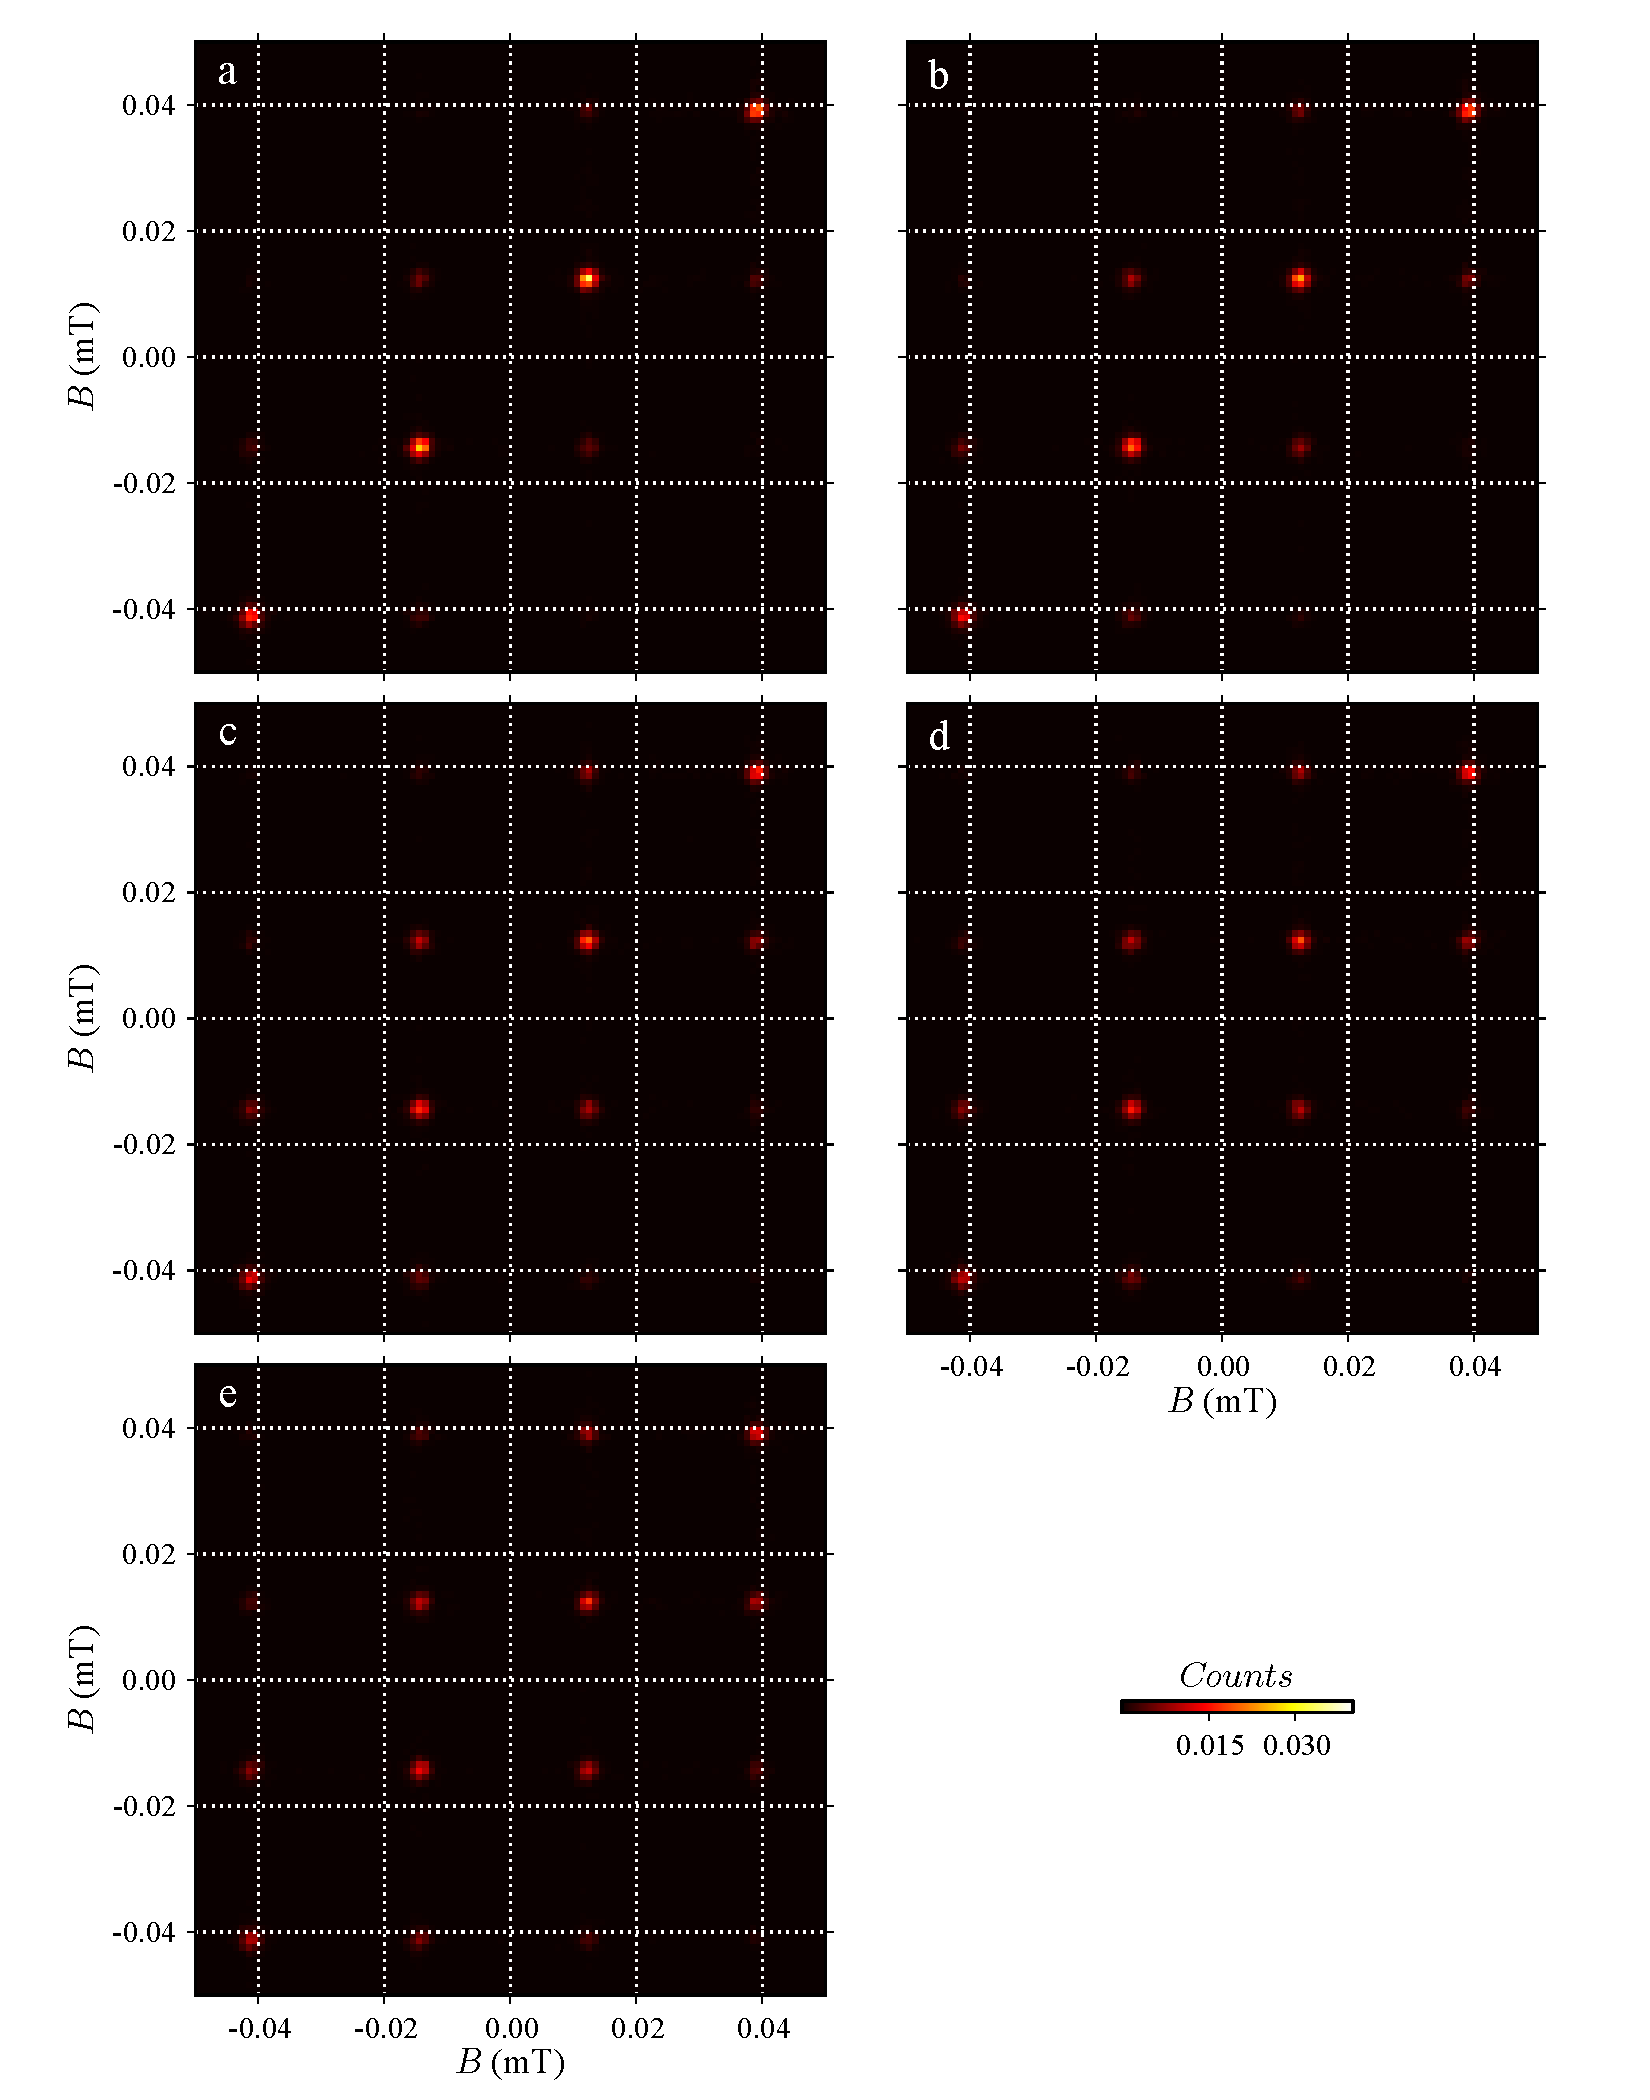
\includegraphics[scale=0.45]{Resultats/MesureInfl/MesureInfl.pdf} 
\caption{La cartographie a (b, c, d et e) présente un histogramme 2D rendant compte de la corrélation entre les états de spin nucléaire après deux (trois, quatre, cinq et six) mesures. On constate qu'après six mesures, les éléments diagonaux sont toujours dominant démontrant ainsi le faible influence de notre procédure de mesure sur l'état du spin nucléaire.}
\label{evolution_mesures}
\end{figure}

\subsection{Extraction des populations nucléaires}
Au chapitre précédent, nous avons montré qu'à travers un histogramme des positions en champ des renversements, on pouvait facilement identifier les différents états de spin.Nous allons utiliser cette m\^eme mesure en la présentant différemment. En effet, chaque retournement au voisinage d'une résonance peut \^etre attribuée à un état de spin précis, les différents résonances ne se recouvrant pas. En intégrant et en normalisant le nombre de mesures obtenues pour chaque état de spin nucléaire, on peut reconstruire leur distribution. C'est ce qui est présenté dans la Fig. \ref{extract_pop} ou l'histogramme original est montré en \textbf{a} et la population qui en est extraite en \textbf{b}.

Cependant, cette dernière contient en fait deux distributions, l'une relative à $J_z=-6$ et l'autre à $J_z=+6$ comme nous l'avons déjà montré. Il est cependant possible de les différencié à partir du signe du changement en conductance relatif à chaque mesure $\Delta g$. Dans la suite, du fait d'un initialisation à champ négatif, nous prendrons toujours pour référence la situation où $J_z=-6$ car il s'agit de l'état fondamental, donc plus probable, et il fournis donc une meilleure statistique.

\begin{figure}
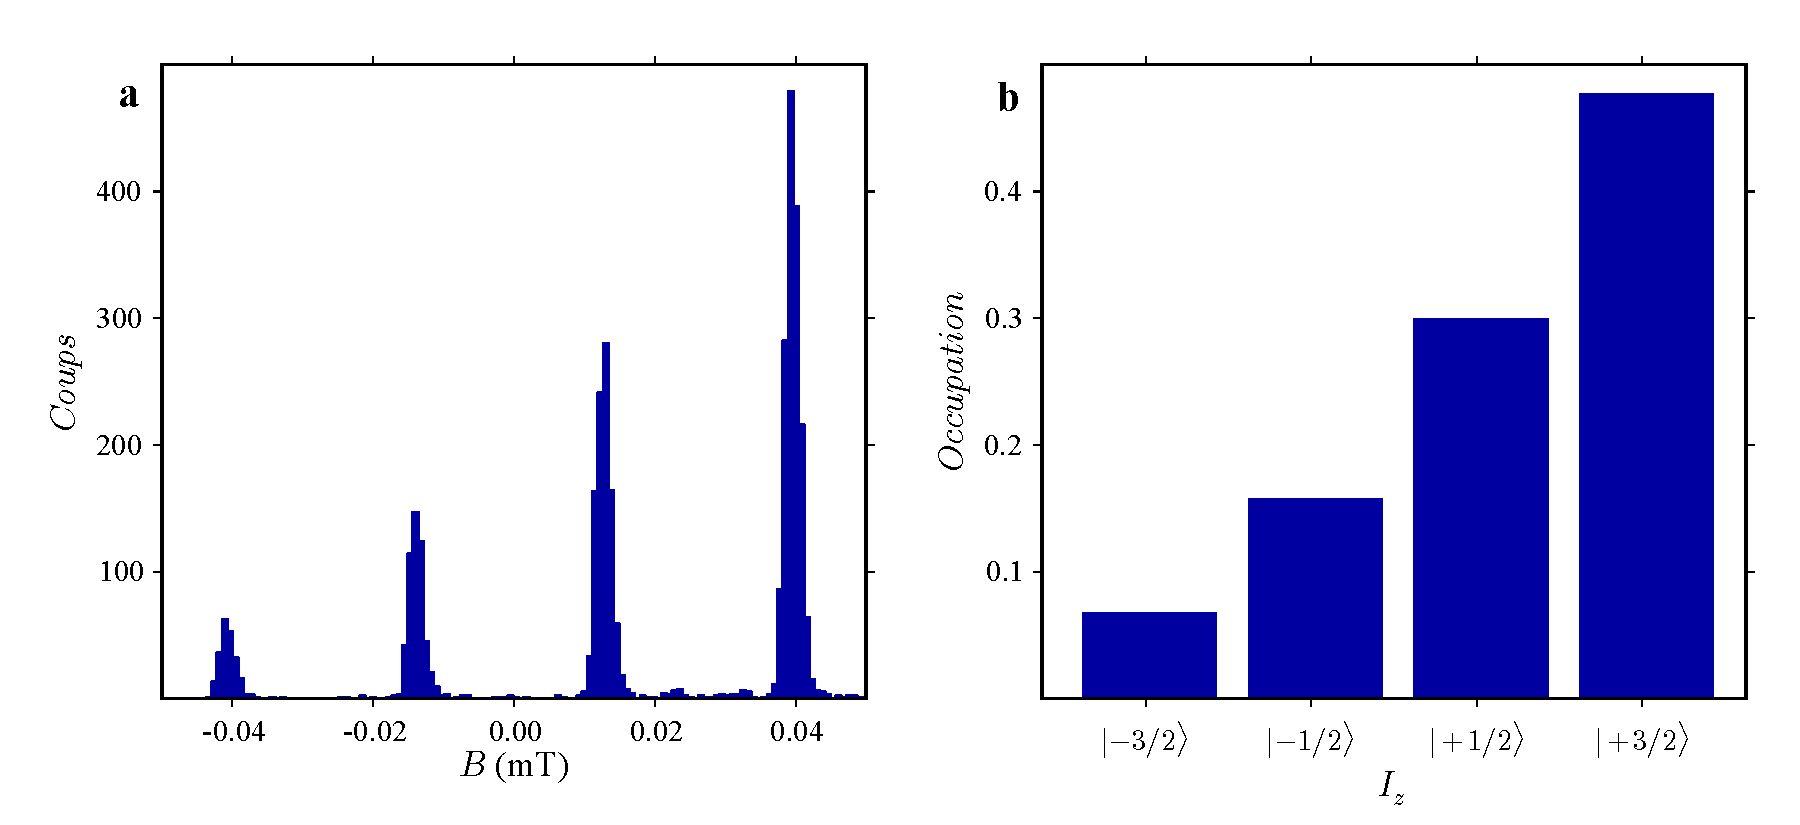
\includegraphics[scale=0.45]{Resultats/PopState/PopState.pdf} 
\caption{\textbf{a -} Histogramme des champs de retournement obtenue durant la trace et correspondant à la transition $J_z = +6 \rightarrow -6$. \textbf{b -} Population des états de spin nucléaire obtenue à partir de l'histogramme présenté en \textbf{a}. Du fait de la relaxation, on constate la prédominance de l'état fondamental $I_z=+3/2$ sur les autres états.}
\label{extract_pop}
\end{figure}

Nous allons maintenant utiliser cette technique d'extraction des populations pour étudier son évolution en fonction du temps pour deux environnements électrostatiques différents.

\subsection{Influence de la tension de grille sur la relaxation}
Afin d'évaluer l'influence de la tension de grille sur la relaxation, nous avons mesuré l'évolution de la population des états de spin en fonction du temps pour deux points polarisation ($V_g$,$V_{ds}$) différent : ($-0.9\, V$,$0\, V$) et ($-0.1\, V$,$0\, V$). Pour chacun de ces points nous avons fait varié le temps d'attente entre la retrace et la trace suivante de 0, 5, 10, 20 et 50 secondes et la population des états nucléaire a été reconstruite à partir des transitions obtenues durant la trace, en sélectionnant seulement celles correspondant à l'état fondamental $J_z=+6$.

La Fig.\ref{dynamique_spin}.\textbf{a} et \textbf{b} présentent les résultats obtenus. On constate immédiatement que les deux distribution évolue différemment. Pour la tension de grille $V_g = -0.9V$ la relaxation vers l'équilibre thermodynamique se fait plus lentement que lorsque $V_g = -0.1V$.  Ceci peut s'expliquer par la modification du courant circulant à travers le système du fait de la modification de la tension de grille. Celle-ci entraîne un changement dans les fluctuations de champ électrique  qui, en se couplant au moment quadripolaire du spin nucléaire, vont modifier les processus de relaxation.

Un analyse plus fine en grille n'a cependant pas permis déterminer le phénomène physique rendant compte de cette dépendance.

\subsection{Détermination de la température nucléaire}
La température du spin nucléaire a également été mesuré. Pour cela, nous avons choisi de nous placer sur le second point de fonctionnement pour lequel l'équilibre est atteint plus rapidement, ce qui nous  a permis de choisir un temps d'attente relativement faible pour effectuer notre étude. En effet, au vu du nombre de mesures nécessaire (22000 mesures), on ne peut pas attendre le temps nécessaire à l'équilibre thermodynamique. Nous avons choisi un compromis en prenant un temps d'attente de 10 secondes. Bien attendu, comme le montre l'étude précédente, l'abscence d'équilibre ne nous permet pas de déduire, directement à partir de la distribution, la température du spin nucléaire.

Pour contourner cette limitation, nous avons choisi d'utiliser une méthode indirecte. Pour cela, la distribution des état nucléaire a été mesuré pour plusieurs température. La distribution observé pour $100\,mK$ a servie de référence, car celle-ci est très proche de la température électronique ($\sim 80\,mK$). La distribution ne va différé de la distribution de référence qu'à condition que la température imposé au système soit supérieur à la température nucléaire de référence obtenue à $100\,mK$.

\begin{figure}[h!]
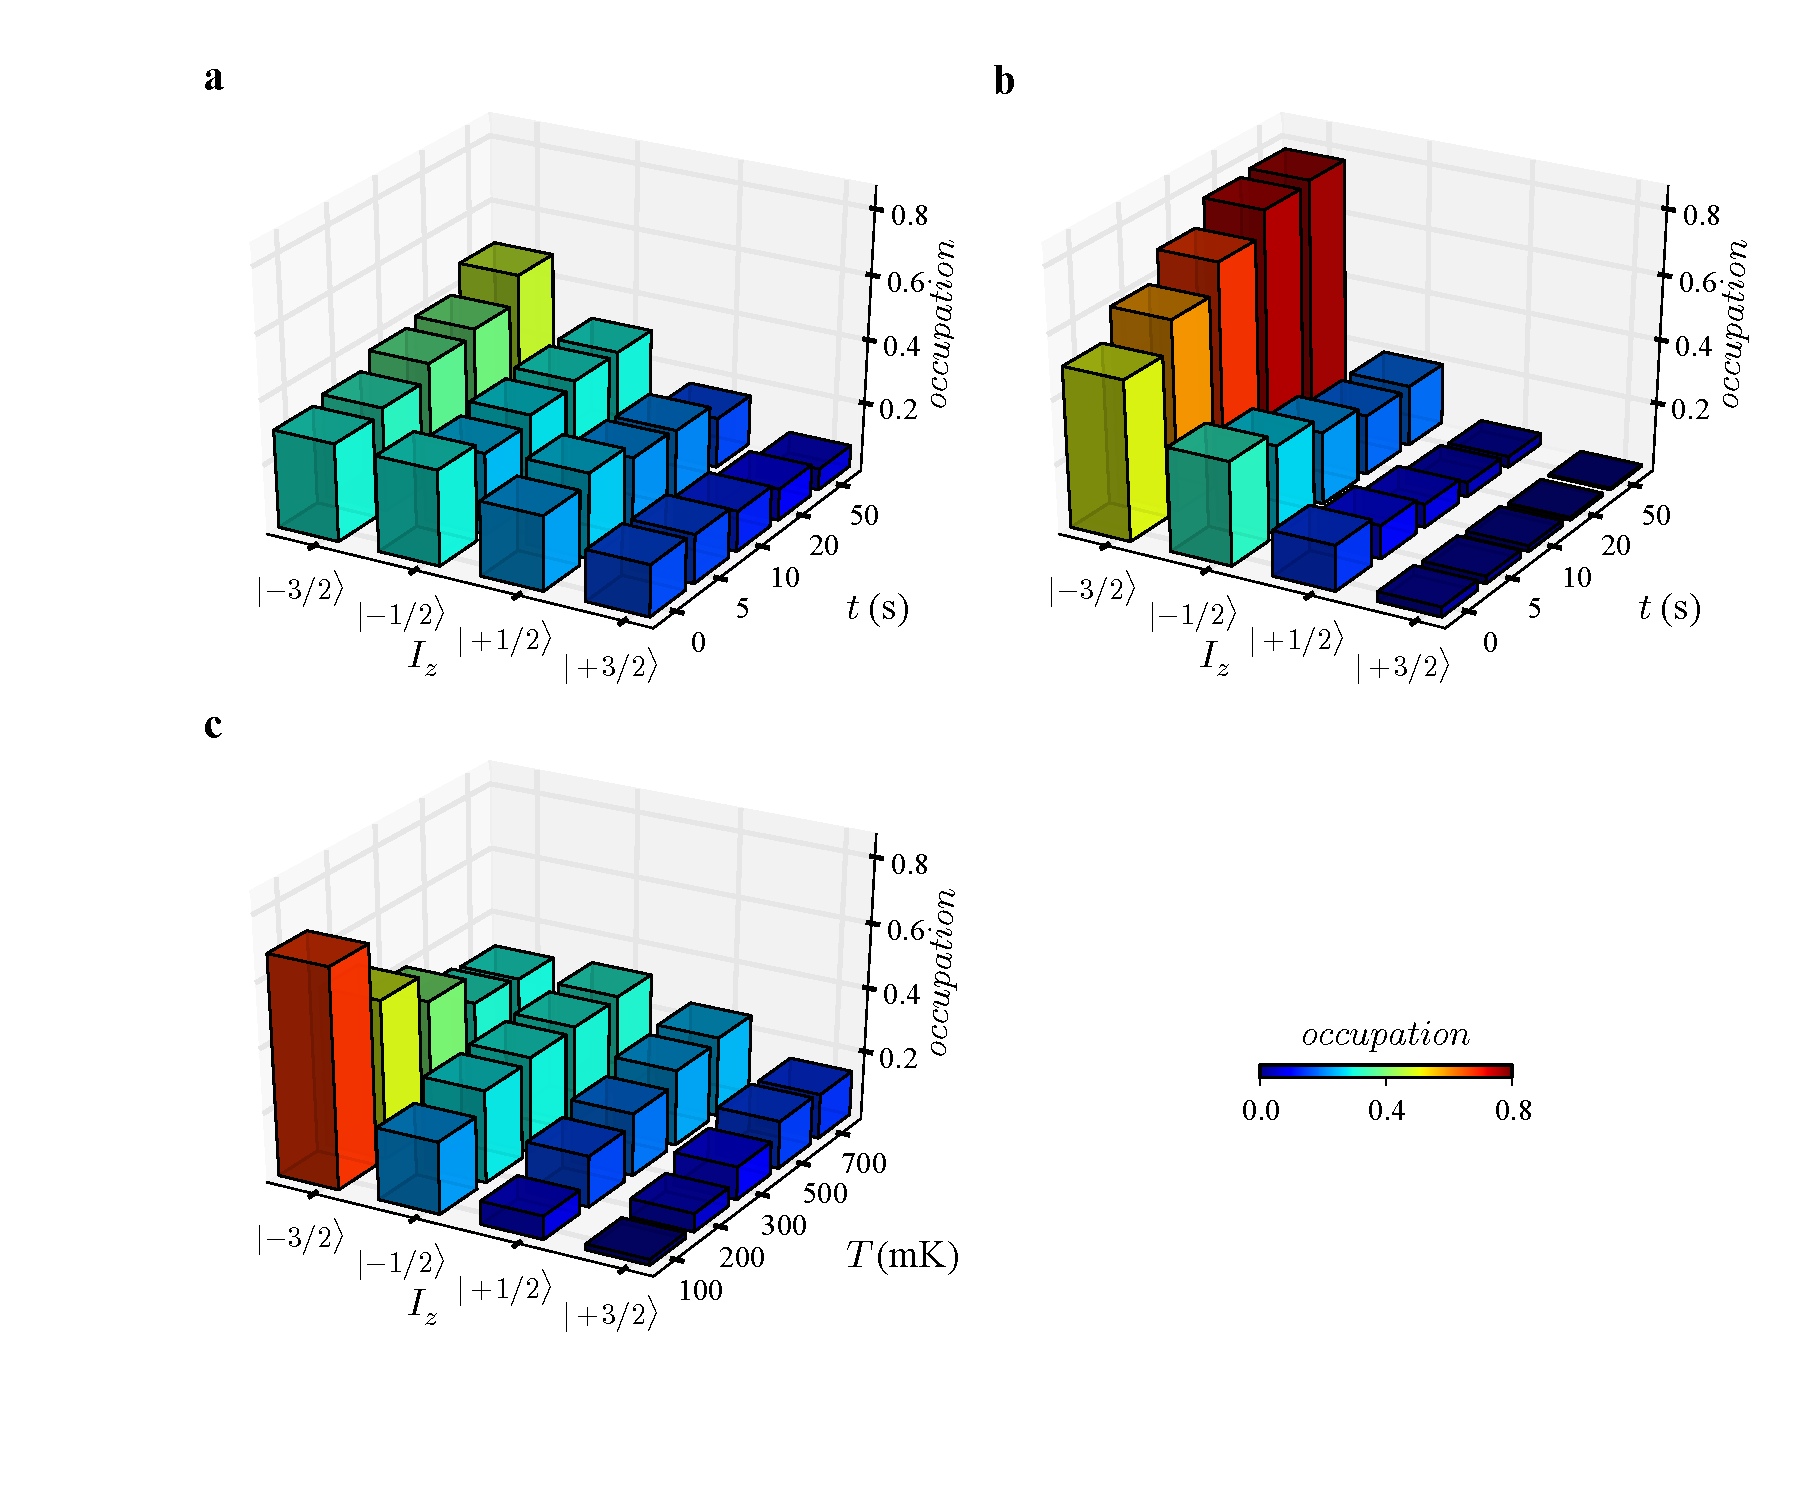
\includegraphics[scale=0.45]{Resultats/SpinTemp/SpinTemp.pdf} 
\caption{Evolution de la population des états nucléaire pour deux points de fonctionnement différent : \textbf{a}, $V_g = -0.9\,V$; et \textbf{b}, $V_g = -0.1\,V$ (avec à chaque fois $V_{ds} = 0\,V$. Ces deux mesures montrent clairement que le système évolue vers deux équilibres thermodynamique différent. \textbf{c}, dynamique du spin nucléaire pour un temps d'attente de 10 secondes, en fonction de la température $T$. Lorsque l'on augmente la température, la population des états de spin nucléaire évolue vers une occupation égale de tous les états.}
\label{dynamique_spin}
\end{figure}


La Fig.\ref{dynamique_spin}.\textbf{c} présente l'évolution de la distribution à $10\,$ seconde en fonction de la température. La distribution évolue entre 100 et 200$\,mK$ et celle-ci est largement modifié pour $T\geq 300mK$. Les états de plus hautes énergies commencent à se peupler pour tendre vers l'équiprobabilité vers $T=700\,mK$. On peut donc en déduire qu'à la température de base, la température d'équilibre du spin nucléaire se situe entre 100 et 200 $\,mK$, preuve que le spin nucléaire peut être refroidi de manière efficace. En effet, cette température d'équilibre est très proche de la température électronique de notre système évalué autour de $100\,mK$.
%\subsection{Perspectives}